\clearpage
\phantomsection\addcontentsline{toc}{section}{报告 III B --- 局部项的计算}
\section*{报告 III B\\局部项的计算}
\begin{center}
Luc Illusie 著
\end{center}

\section*{引言}

本报告写于 1977 年 1 月, 并不对应讨论班中的任何一次口头报告. 它由两个彼此独立的部分组成. 第一部分计算代数闭域上光滑曲线之间的上同调对应的 Lefschetz--Verdier 局部项, 这些对应支承于满足某些一般位置假设的对应上. 所得公式的推论包括 Verdier 关于横截自同态的公式~[6] (特别适用于 Frobenius 自同态), 以及 Langlands 在 ([4]~7.12) 中陈述的公式. 证明方法与 Artin--Verdier 在 [6] 中采用的方法平行. 我们将问题归结为: 当给定层复形在所考察不动点的各像处的纤维为零时, 证明局部项消失; 实际上证明一个更强的性质, 即某个限制映射为零 (2.5). 为此, 先对两条给定曲线作相同次数的覆盖, 以免破坏一般位置假设, 将问题归结为温和分歧的情形, 再用 Abhyankar 引理和相对纯性定理直接处理该情形. 第二部分在技术上复杂得多, 其灵感来自 Grothendieck 用于建立曲线上某些上同调对应的 Lefschetz 公式的方法 (见 XII 及 (SGA~$4^{1/2}$ Rapport)). 第~5 节对拓扑斯上的模复形建立非交换迹理论, 推广 (SGA~6~I) 的交换理论; 对点拓扑斯, 它恢复 Grothendieck 在口头讨论班中建立的非交换理论 (该理论曾整理为报告 XI, 遗憾的是已经遗失). 第~6 节运用第~5 节的技术, 对不必交换的环上的模复形之间的上同调对应定义 Lefschetz--Verdier 局部项. 这些局部项具有非交换迹的性质, 特别地, 当基环取为群代数时, 可将等变对应的通常局部项作典范的整除. 作为应用, 我们以更一般的形式证明 Grothendieck 在 (XII~4.5) 中提出的整除性猜想. 我们还证明 Grothendieck 在 XII 的 Lefschetz 公式中定义的局部项确为 Lefschetz--Verdier 局部项, 并推广该处的公式.

感谢 P.~Deligne 在多次讨论中提出的有益建议; 尤其感谢他指出定理~1.2 的一个早期证明中的错误, 并帮助我改正.

\section*{内容提要}
\begin{tabular}{@{}p{0.84\textwidth}r@{}}
I. 曲线之间处于一般位置的对应 & 3\\
1. 定理及其推论的陈述 & 3\\
2. 归结为一个消失定理 & 9\\
3. 归结为温和情形 & 15\\
4. 完成 1.2 的证明 & 20\\
II. 等变对应 & 25\\
5. 非交换迹 & 25\\
6. 等变对应与局部项的整除性 & 46
\end{tabular}

\section*{I. 曲线之间处于一般位置的对应}

本部分中, $S$ 表示特征为 $p$ 的代数闭域 $k$ 的谱, $\Lambda$ 是被某个与 $p$ 互素的整数零化的 Noether 交换环. 对每个 $S$ 上的概形 $X$, 用 $D(X)$ 表示 $X$ 上的 $\Lambda$-模层的导出范畴, 用 $D_{\ctf}(X)$ 表示 $D(X)$ 中由具有有限 Tor 维数和可构造上同调的复形组成的满子范畴.

\subsection*{1. 定理及其推论的陈述}

\subsubsection*{1.1}
设 $X$ (相应地 $Y$) 是一条光滑分离 $S$-曲线在某个闭点处的严格局部化, $A$ (相应地 $B$) 是严格局部 $S$-概形, 且
\[
a:A\longrightarrow X\times_S Y,
\qquad
b:B\longrightarrow X\times_S Y
\]
是 $S$-态射. 以 $p_1:X\times_S Y\to X$, $p_2:X\times_S Y\to Y$ 表示投影, 置 $a_i=p_i a$, $b_i=p_i b$, 并以 $x$ (相应地 $y$) 表示 $X$ (相应地 $Y$) 的闭点. 假定 $a_2$ 和 $b_1$ 有限且满射, 而 $A\times_{(X\times_S Y)}B$ 仅由闭点 $z$ 组成, 该点在 $X\times_S Y$ 中的像为 $(x,y)$.

设 $L\in \ob D_{\ctf}(X)$, $M\in \ob D_{\ctf}(Y)$, $u\in\Hom(a_1^*L,a_2^!M)$, $v\in\Hom(b_2^*M,b_1^!L)$. 用
\[
u_z\in\Hom(L_x,M_y)\qquad (\text{相应地 }v_z\in\Hom(M_y,L_x))
\]
表示复合同态
\[
L_x=R\Gamma(X,L)\xrightarrow{a_1^*}R\Gamma(A,a_1^*L)
\xrightarrow{R\Gamma(A,u)}R\Gamma(A,a_2^!M)
\xrightarrow{a_{2*}}R\Gamma(Y,M)=M_y,
\]
其中 $a_{2*}$ 由伴随映射 $a_{2*}a_2^!M\to M$ 定义 (相应地, 用 $(b,v)$ 定义类似的复合同态). 因 $L_x$ 和 $M_y$ 是 $\Lambda$-模的完美复形, 可作杯积 (SGA~6~I~8.3)
\begin{equation}\tag{1.1.1}
\langle u_z,v_z\rangle=\Tr(u_zv_z)=\Tr(v_zu_z)\in\Lambda.
\end{equation}
置 $\Lambda_X(1)[2]=K_X$, $\Lambda_Y(1)[2]=K_Y$. 由 (I~5) (或 (SGA~$4^{1/2}$ Duality~1, 或 Finitude~4.1)), $D_{\ctf}(X)$ (相应地 $D_{\ctf}(Y)$) 上的函子 $D_X=\RHom(-,K_X)$ (相应地 $D_Y=\RHom(-,K_Y)$) 是对偶化函子, 即对每个 $E\in\ob D_{\ctf}(X)$ (相应地 $E\in\ob D_{\ctf}(Y)$), 有 $E\xrightarrow{\sim}D_XD_XE$ (相应地 $E\xrightarrow{\sim}D_YD_YE$). 有时简写 $D$ 代替 $D_X$, $D_Y$.

另一方面, 用 $p_i^!$ 表示函子 $p_i^*(-)(1)[2]$. 显然有
\[
K_X\otimes_S^{\LL}M\xrightarrow{\sim}p_2^!M,
\qquad
L\otimes_S^{\LL}K_Y\xrightarrow{\sim}p_1^!L,
\]
由 (III~2.3) 取极限可知, 类似于 (III~3.1.1) 的 Künneth 映射
\[
DL\otimes_S^{\LL}M\longrightarrow \RHom(p_1^*L,p_2^!M),
\qquad
L\otimes_S^{\LL}DM\longrightarrow \RHom(p_2^*M,p_1^!L)
\]
都是同构. 因 $a_2$ 有限, $a$ 亦有限, 所以函子 $a^!$ 有定义; 容易验证有传递性同构 $a^!p_2^!=a_2^!$. 因而由 $a$ 的诱导公式 (SGA~4~XVIII~3.1.12.2), 有类似于 (III~3.2.1) 的典范同构
\[
a^!\RHom(p_1^*L,p_2^!M)\xrightarrow{\sim}\RHom(a_1^*L,a_2^!M),
\]
从而得到同构
\begin{equation}\tag{*}
\Hom(a_1^*L,a_2^!M)\xrightarrow{\sim}H^0(X\times_S Y,a_*a^!(DL\otimes_S^{\LL}M)).
\end{equation}
同样有同构
\begin{equation}\tag{**}
\Hom(b_2^*M,b_1^!L)\xrightarrow{\sim}H^0(X\times_S Y,b_*b^!(L\otimes_S^{\LL}DM)).
\end{equation}
如同 (III~4.1.2), 定义自然配对
\[
(DL\otimes_S^{\LL}M)\otimes^{\LL}(L\otimes_S^{\LL}DM)
\longrightarrow K_X\otimes_S^{\LL}K_Y=\Lambda_{X\times_S Y}(2)[4]\stackrel{\mathrm{dfn}}{=}K_{X\times_S Y}.
\]
再与类似于 (III~4.2.3) 的配对复合
\[
a_*a^!P\otimes^{\LL} b_*b^!Q\longrightarrow c_*c^!(P\otimes^{\LL}Q),
\]
其中 $P=DL\otimes_S^{\LL}M$, $Q=L\otimes_S^{\LL}DM$, 而 $c:Z=A\times_{(X\times_S Y)}B\to X\times_S Y$ 为典范投影; 结合同构 (*), (**), 可得类似于 (III~4.2.5) 的配对
\[
\langle\ ,\ \rangle:\Hom(a_1^*L,a_2^!M)\otimes\Hom(b_2^*M,b_1^!L)
\longrightarrow H^0(X\times_S Y,c_*c^!K_{X\times_S Y}).
\]
取极限容易验证 $c^!K_{X\times_S Y}=\Lambda_z$, 因而 $H^0(X\times_S Y,c_*c^!K_{X\times_S Y})=\Lambda$. 于是有一个``杯积''
\begin{equation}\tag{1.1.2}
\langle u,v\rangle\in\Lambda.
\end{equation}

\subsubsection*{1.1.3}
设 $X'$ (相应地 $Y'$) 是光滑 $S$-曲线, $A'$ (相应地 $B'$) 是分离 $S$-曲线,
\[
a':A'\longrightarrow X'\times_S Y',
\qquad
b':B'\longrightarrow X'\times_S Y'
\]
为有限 $S$-态射, $x'$ (相应地 $y'$) 为 $X'$ (相应地 $Y'$) 的闭点, $z'$ 为 $A'\times_{(X'\times_S Y')}B'$ 的孤立闭点, 在 $A'$ (相应地 $B'$) 中的像为 $s'$ (相应地 $t'$), 并且 $a'_2(=p_2a')$ (相应地 $b'_1(=p_1b')$) 在 $s'$ (相应地 $t'$) 处拟有限,
\[
L'\in\ob D_{\ctf}(X'),\quad M'\in\ob D_{\ctf}(Y'),\quad
u'\in\Hom(a_1'^*L',a_2'^!M'),\quad v'\in\Hom(b_2'^*M',b_1'^!L').
\]
此时可考虑局部项 (III~4.2.7) $\langle u',v'\rangle_{z'}\in\Lambda$. 另一方面, 若 $X,Y,A,B$ 为 $X',Y',A',B'$ 在 $x',y',s',t'$ 处的严格局部化, $a:A\to X\times_S Y$, $b:B\to X\times_SY$ 为由 $a'$, $b'$ 导出的态射, $L=L'|X$, $M=M'|Y$, 且 $u\in\Hom(a_1^*L,a_2^!M)$, $v\in\Hom(b_2^*M,b_1^!L)$ 为由 $u'$, $v'$ 导出的映射, 则数据 $(X,Y,a,b,u,v)$ 满足 1.1 开头的假设, 因此杯积 1.1.2 $\langle u,v\rangle\in\Lambda$ 有定义. 局部项的构造 (III~4.2.7) 与局部化相容 (III~4.2.6), 故 $\langle u',v'\rangle_{z'}=\langle u,v\rangle$. 也容易看出, 满足 1.1 开头假设的任意数据 $(X,Y,a,b,u,v)$ 都由上述形式的数据 $(X',Y',a',b',x',y',z',s',t',u',v')$ 诱导; 如有需要, 还可假定 $A'\times_{(X'\times_S Y')}B'$ 仅由 $z'$ 组成.

一般而言, 杯积 1.1.1 和 1.1.2 并不相等. 不过有下述定理, 它是本部分的主要结果:

\begin{statement}{定理 1.2}
在 1.1 开头的假设下, 再假定 $A$ 与 $B$ 处于一般位置, 即二者在 $X\times_S Y$ 中的像在 $(x,y)$ 处的切锥之交仅为 $(x,y)$; 同样假定 $A$ 与 $X\times\{y\}$ 以及 $\{x\}\times Y$ 与 $B$ 处于一般位置. 则
\begin{equation}\tag{1.2.1}
\langle u_z,v_z\rangle=\langle u,v\rangle.
\end{equation}
\end{statement}

由 Lefschetz--Verdier 公式 (III~4.7), 结合 1.1.3, 得到:

\begin{statement}{推论 1.3}
设 $F$ 是固有光滑曲线 $X/S$ 的自同态, 不动点概形 $X^F$ 有限, 且由 $F$ 的图像与对角线横截之处的点组成. 设 $L\in\ob D_{\ctf}(X)$, $u\in\Hom(F^*L,L)$. 则
\[
\Tr((F,u),R\Gamma(X,L))=\sum_{x\in X^F}\Tr(u_x,L_x),
\]
其中两端的迹均按 (SGA~6~I~8) 的意义理解.
\end{statement}

当 $L$ 集中于 $0$ 次时, 1.3 即 Artin--Verdier 的结果 ([6]~4.1). 用 XV 中说明的取极限方法, 可由 1.3 推出 $\ell$ 进上同调中的类似结果 ([6]~1.1), (XV~\S2 第~3 小节命题~2):

\begin{statement}{推论 1.3.1}
设 $X$ 和 $F$ 如 1.3, $L$ 是 $X$ 上的可构造 $\mathbb Q_\ell$-层 ($\ell$ 与 $p$ 互素), $u\in\Hom(F^*L,L)$. 则:
\[
\sum_i(-1)^i\Tr((F,u),H^i(X,L))=\sum_{x\in X^F}\Tr(u_x,L_x).
\]
\end{statement}

1.3 和 1.3.1 的假设特别适用于 $(F,u)$ 是 Frobenius 对应 (XV~2) 的情形, 从而得到 Grothendieck 的迹公式 ([2]~5.1), (SGA~$4^{1/2}$ Rapport~3.2).

\subsubsection*{1.4}
沿用 1.1 的记号, 假定 $b_2$ 和 $a_1$ 有限且满射 (代替 $a_2$ 和 $b_1$), 并考虑对偶对应 (III~5.1)
\[
Du\in\Hom(a_2^*DM,a_1^!DL),\qquad Dv\in\Hom(b_1^*DL,b_2^!DM),
\]
以及同态 $(Du)_z\in\Hom((DM)_y,(DM)_x)$, $(Dv)_z\in\Hom((DL)_x,(DM)_y)$. 假定 $(A,\{x\}\times Y)$, $(X\times\{y\},B)$ 和 $(A,B)$ 均处于一般位置. 对 $Du,Dv$ 应用 1.2, 得
\[
\langle Du,Dv\rangle=\langle (Du)_z,(Dv)_z\rangle,
\]
从而由 (III~5.1.6) 和 (III~4.2.6),
\begin{equation}\tag{1.4.1}
\langle u,v\rangle=\langle (Du)_z,(Dv)_z\rangle.
\end{equation}

由此注及 1.2, 利用 Lefschetz--Verdier 公式 (III~4.7) 得到:

\begin{statement}{推论 1.5}
设 $X,Y$ 是 $S$ 上的固有光滑曲线,
\[
a:A\longrightarrow X\times_S Y,
\qquad
b:B\longrightarrow X\times_S Y
\]
是对应, 其中 $A$ 和 $B$ 为 $S$ 上的固有曲线; 设 $L\in\ob D_{\ctf}(X)$, $M\in\ob D_{\ctf}(Y)$, $u\in\Hom(a_1^*L,a_2^!M)$, $v\in\Hom(b_2^*M,b_1^!L)$. 假定 $C=A\times_{(X\times_S Y)}B$ 在 $S$ 上有限, 并可写成 $C=C_1\amalg C_2$, 满足: 对 $z\in C_1$, 在 $z$ 的各像处严格局部化后由 $a_2,b_1$ 导出的态射有限; 若 $(x,y)$ 表示 $z$ 在 $X\times_S Y$ 中的像, 则 $(A,B)$, $(A,X\times\{y\})$, $(\{y\}\times Y,B)$ 各对均在 $(x,y)$ 处处于一般位置; 对 $z\in C_2$, 在 $z$ 的各像处严格局部化后由 $a_1,b_2$ 导出的态射有限, 且 $(A,B)$, $(A,\{x\}\times Y)$, $(B,X\times\{y\})$ 各对在 $(x,y)$ 处处于一般位置 (``一般位置'' 意为所考察的两条曲线之像在 $(x,y)$ 处的切锥之交仅为 $(x,y)$). 那么, 若 $u_*\in\Hom(R\Gamma(X,L),R\Gamma(Y,M))$, $v_*\in\Hom(R\Gamma(Y,M),R\Gamma(X,L))$ 为 $u,v$ 定义的态射 (III~3.7.6), 用 1.1.1, (III~5.1.5) 的记号, 有
\begin{equation}\tag{1.5.1}
\langle u_*,v_*\rangle=\sum_{z\in C_1}\langle u_z,v_z\rangle+\sum_{z\in C_2}\langle (Du)_z,(Dv)_z\rangle.
\end{equation}
\end{statement}

\subsubsection*{1.6}
假定 $\ell$ 进上同调的形式体系, 用 XIV 的取极限技术可由 1.5 推出: 在 1.5 对 $X,Y,a,b$ 的假设下, 对 $L\in\ob D^b(X,\mathbb Q_\ell)$ ($\ell$ 为不等于 $p$ 的素数), $M\in\ob D^b(Y,\mathbb Q_\ell)$, $u\in\Hom(a_1^*L,a_2^!M)$, $v\in\Hom(b_2^*M,b_1^!L)$, 有 $\mathbb Q_\ell$ 中类似于 1.5.1 的公式. 该公式包含 Langlands [4] 的命题 7.12 作为特例: 应用公式时, 取 $X=Y$, $M$ 为 Langlands 考虑的层 $F$; $L=\alpha M$ ($\alpha\in\mathbb Q_\ell^*$), $A$ 为 $X\times X$ 的对角线, $b$ 为该处的对应 $\phi$, $u$ 为由 $\alpha^{-1}:L\to M$ 给出的支承于 $A$ 的对应, $v$ 为该处的对应 $\Phi$; 用该处的记号, $C_1$ (相应地 $C_2$) 是满足 $a<d$ (相应地 $a>d$) 的不动点之集.

\subsubsection*{1.7}
在 1.2 的假设下, 取 $u$ (相应地 $v$) 为 $\Tr_{a_2}:a_{2*}\Lambda\to\Lambda$ (相应地 $\Tr_{b_1}:b_{1*}\Lambda\to\Lambda$) 定义的对应 $\cl(A)$ (相应地 $\cl(B)$). 公式 1.2.1 化为
\begin{equation}\tag{1.7.1}
\deg(a_2)\deg(b_1)=\langle \cl(A),\cl(B)\rangle,
\end{equation}
其中 $\deg(a_2)$ (相应地 $\deg(b_1)$) 表示 $a_2$ (相应地 $b_1$) 的一般次数. 考虑到一般位置假设, 1.7.1 的左端正是闭链 $a_*A$, $b_*B$ 在 $(x,y)$ 处的相交重数, 这里它们是 $A$ 和 $B$ 的正像. 利用闭链的上同调类的构造与相交的相容性 (SGA~$4^{1/2}$ Cycle~2.3.8), 不难直接推出 1.7.1.


\subsection*{2. 归结为一个消失定理}

\subsubsection*{2.1}
在 1.1 的假设下, 以 $s$ (相应地 $t$) 表示 $z$ 在 $A$ (相应地 $B$) 中的像, 以 $i:U=X-\{x\}\hookrightarrow X$ 和 $j:V=Y-\{y\}\hookrightarrow Y$ 表示典范包含. 因 $a_2$ 与 $b_1$ 有限, 有 $a_2^{-1}(y)=s$, $b_1^{-1}(x)=t$, 所以
\[
a_1^{-1}(U)\subset a_2^{-1}(V),\qquad b_2^{-1}(V)\subset b_1^{-1}(U),
\]
并有交换图
\[
\begin{tikzcd}[column sep=large,row sep=large]
U \arrow[d,"i"] \arrow[rd,phantom,"(1)"{description}] & a_1^{-1}(U) \arrow[l,"a'_1"'] \arrow[r,"a'_2"] \arrow[d] \arrow[rd,phantom,"(2)"{description}] & V \arrow[d,"j"]\\
X & A \arrow[l,"a_1"] \arrow[r,"a_2"'] & Y
\end{tikzcd}
\qquad
\begin{tikzcd}[column sep=large,row sep=large]
U \arrow[d,"i"] \arrow[rd,phantom,"(3)"{description}] & b_2^{-1}(V) \arrow[l,"b'_1"'] \arrow[r,"b'_2"] \arrow[d] \arrow[rd,phantom,"(4)"{description}] & V \arrow[d,"j"]\\
X & B \arrow[l,"b_1"] \arrow[r,"b_2"'] & Y ,
\end{tikzcd}
\]
其中方块 (1) 和 (4) 为笛卡尔方块.

\begin{statement}{引理 2.2}
为证明 1.2, 只需考虑以下两种情形:
\[
\text{a) } L_x=0,\quad M_y=0;\qquad
\text{b) } L|U=0,\quad M|V=0 .
\]
\end{statement}

考虑 $L$ 和 $M$ 上由以下子复形定义的递减滤过
\[
F^nL=
\begin{cases}
L,& n\le 0,\\
i_!i^*L,& n=1,\\
0,& n>1,
\end{cases}
\qquad
F^nM=
\begin{cases}
M,& n\le 0,\\
j_!j^*M,& n=1,\\
0,& n>1.
\end{cases}
\]
于是复形 $a_{2*}a_1^*L$ (相应地 $b_{1*}b_2^*M$) 的滤过为
\[
F^n a_{2*}a_1^*L=a_{2*}a_1^*F^nL.
\]
对 $n\le0$, 有 $F^n a_{2*}a_1^*L=a_{2*}a_1^*L$; 对 $n>1$, 则为 $0$; 又因 $a_2$ 有限且方块 (1) 为笛卡尔方块,
\[
F^1a_{2*}a_1^*L=j_!(a'_2)_!(a'_1)^*i^*L.
\]
类似地,
\[
F^n b_{1*}b_2^*M=
\begin{cases}
b_{1*}b_2^*M,& n\le 0,\\
i_!(b'_1)_!(b'_2)^*j^*M,& n=1,\\
0,& n>1.
\end{cases}
\]

可假定 $u$ (相应地 $v$) 由复形同态定义
\[
u:a_{2*}a_1^*L\longrightarrow M
\quad
(\text{相应地 }v:b_{1*}b_2^*M\longrightarrow L).
\]
以上公式表明复合
\[
F^1a_{2*}a_1^*L\longrightarrow a_{2*}a_1^*L\xrightarrow{u}M
\]
(相应地 $F^1b_{1*}b_2^*M\to b_{1*}b_2^*M\xrightarrow{v}L$) 唯一地经由 $F^1M$ (相应地 $F^1L$) 分解; 换言之, $u$ (相应地 $v$) 是滤过复形同态. 因此 $u$ (相应地 $v$) 是一个 (III 4.13) 意义下的滤过对应的底层对应, 仍记作
\[
u\in\Hom_{DF}(a_1^*L,a_2^!M),\qquad
v\in\Hom_{DF}(b_2^*M,b_1^!L).
\]
由杯积的可加性 ([3] V 3.8.7), (III 4.13.1), 有
\[
\langle u_z,v_z\rangle
 =\langle \operatorname{gr}^0u_z,\operatorname{gr}^0v_z\rangle
 +\langle \operatorname{gr}^1u_z,\operatorname{gr}^1v_z\rangle,
\]
以及
\[
\langle u,v\rangle
 =\langle \operatorname{gr}^0u,\operatorname{gr}^0v\rangle
 +\langle \operatorname{gr}^1u,\operatorname{gr}^1v\rangle.
\]
由于 $\operatorname{gr}^1L=i_!i^*L$ (相应地 $\operatorname{gr}^1M=j_!j^*M$) 在 $x$ (相应地 $y$) 处的纤维为零, 而 $\operatorname{gr}^0L$ (相应地 $\operatorname{gr}^0M$) 集中于 $x$ (相应地 $y$), 引理即得证.

\begin{statement}{引理 2.3}
在 1.1 的假设下, 假定 $L|U=0$, $M|V=0$. 则
\[
\langle u_z,v_z\rangle=\langle u,v\rangle .
\]
\end{statement}

证明的思路是: 此时 $u$ 和 $v$ 是集中于闭点的复形之间的对应的正像, 所要证明的公式仅是投影 $x\to S$, $y\to S$ 的 Lefschetz 公式. 根据 1.1.3, 可将 1.1 的数据替换为: $X$ (相应地 $Y$) 是带有闭点 $x$ (相应地 $y$) 的光滑 $S$-曲线, $A$ (相应地 $B$) 是分离 $S$-曲线, $a:A\to X\times_S Y$, $b:B\to X\times_S Y$ 是有限 $S$-态射, 使得 $A\times_{X\times_SY}B$ 仅由 $(x,y)$ 上方的闭点 $z$ 组成,
\[
u\in\Hom(a_1^*L,a_2^!M),\qquad v\in\Hom(b_2^*M,b_1^!L),
\]
其中
\[
L=h_{1*}L',\quad M=h_{2*}M',\quad
L'\in\Ob D_{\mathrm{ctf}}(\{x\}),\quad M'\in\Ob D_{\mathrm{ctf}}(\{y\}),
\]
这里 $h_1:\{x\}\to X$ 和 $h_2:\{y\}\to Y$ 是典范包含. 须证明
\[
\langle u_z,v_z\rangle=\langle u,v\rangle_z,
\]
其中
\[
u_z\in\Hom(\mathrm R\Gamma(X,L),\mathrm R\Gamma(Y,M)),\qquad
v_z\in\Hom(\mathrm R\Gamma(Y,M),\mathrm R\Gamma(X,L))
\]
按 1.1 定义, 而 $\langle u,v\rangle_z$ 是杯积 (III 4.2.7) 在 $z$ 处的值. 有 $\mathrm R\Gamma(X,L)=\mathrm R\Gamma_c(X,L)=L_x$, $\mathrm R\Gamma(Y,M)=\mathrm R\Gamma_c(Y,M)=M_y$; 由计算过程 (III 3.5 b)) 可知, $u_z$ (相应地 $v_z$) 正是 (III 3.7.6) 意义下 $u$ (相应地 $v$) 在 $S$ 上的正像 $u_*$ (相应地 $v_*$).

另一方面, 若 $h=h_1\times_Sh_2:(x,y)\to X\times_SY$ 为包含, 且 $a':A'\to(x,y)$, $b':B'\to(x,y)$ 表示 $a$, $b$ 在 $(x,y)$ 处的纤维, 每个纤维都仅由一点组成, 则有典范同构
\[
h_*a'_*a'{}^!(DL_x\lten_{\Lambda}M_y)
 \xrightarrow{\sim} a_*a^!(DL\lten_{\Lambda}M),
\]
\[
h_*b'_*b'{}^!(L_x\lten_{\Lambda}DM_y)
 \xrightarrow{\sim} b_*b^!(L\lten_{\Lambda}DM),
\]
而箭头
\[
h_*:\Hom(a_1'{}^*L_x,a_2'{}^!M_y)\to \Hom(a_1^*L,a_2^!M),
\]
\[
h_*:\Hom(b_2'{}^*M_y,b_1'{}^!L_x)\to \Hom(b_2^*M,b_1^!L)
\]
(III 3.7.6) 均为同构. 因此对应 $u$ 与 $v$ 唯一地写成
\begin{equation}\tag{1}
u=h_*u',\qquad v=h_*v',
\end{equation}
其中
\[
u'\in\Hom(a_1'{}^*L_x,a_2'{}^!M_y),\qquad
v'\in\Hom(b_2'{}^*M_y,b_1'{}^!L_x).
\]
由 $(h_1,h_2,A'\to A,B'\to B)$ 的 Lefschetz 公式 (III 4.5.1), 有
\begin{equation}\tag{2}
\langle u,v\rangle_z=\langle u',v'\rangle_z .
\end{equation}
另一方面, 由 (1) 有 $u_*=u'_*$ 和 $v_*=v'_*$; 故由 $\{x\}\to S$, $\{y\}\to S$ 的 Lefschetz 公式, 有
\begin{equation}\tag{3}
\langle u_*,v_*\rangle=\langle u',v'\rangle_z .
\end{equation}
结合前面的说明, 比较 (2) 与 (3) 即得结论.

\begin{statement}{引理 2.4}
为证明 1.2, 可假定 $a$ 与 $b$ 为闭浸入, 且只需证明: 若 $L_x=0$ 和 $M_y=0$, 则限制映射
\begin{equation}
H_A^0(X\times_SY,DL\lten_SM)
 \longrightarrow H_z^0(B,b^*(DL\lten_SM))
\tag{2.4.1}
\end{equation}
为零.
\end{statement}

置 $X\times_SY=Z$. $a$ 和 $b$ 的像闭子概形 $a':A'\to Z$, $b':B'\to Z$ 满足与 $a$ 和 $b$ 相同的假设. 设 $u'$ (相应地 $v'$) 是支承于 $A'$ (相应地 $B'$) 的对应, 它是 $u$ (相应地 $v$) 沿伴随箭头 $f_*f^!\to1$ (相应地 $g_*g^!\to1$) 导出的箭头的正像, 其中 $f:A\to A'$ (相应地 $g:B\to B'$) 为投影. 显然 $u_z=u'_z$, $v_z=v'_z$. 另一方面, 由杯积 1.1.2 的定义容易得到
\[
\langle u,v\rangle=\langle u',v'\rangle,
\]
故第一条断言成立.

由 2.2 和 2.3, 可假定 $L_x=0$, $M_y=0$, 此时 1.2 的结论变为 $\langle u,v\rangle=0$. 设 $P,Q\in\Ob D_{\mathrm{ctf}}(Z)$. 杯积
\[
H_A^0(Z,P)\otimes H_B^0(Z,Q)\longrightarrow H_z^0(Z,P\lten Q)
\]
分解为
\[
H_A^0(Z,P)\otimes H_B^0(Z,Q)
 \xrightarrow{\,b^*\otimes 1\,}
H_z^0(B,b^*P)\otimes H_B^0(Z,Q)
 \longrightarrow H_z^0(Z,P\lten Q),
\]
其中 $b^*$ 为限制映射, 第二个箭头是 (SGA $4^{1/2}$ Cycle 1.2.1) 中所考虑乘积的一个变体, 由层截面层次上显然的乘积导出. 例如用 (SGA 4 XVII 4.2) 的松弛预解, 即容易验证此断言. 若 $a':\{z\}\to B$, $b':\{z\}\to A$, $c:\{z\}\to Z$ 为包含, 也可利用 Künneth 箭头 (III 4.2.1)
\[
a'{}^!P\lten_Z b'{}^!Q\longrightarrow c^!(P\lten Q)
\]
的标准分解, 先作``换基箭头''
\[
a'{}^!P\lten_Z b'{}^!Q\longrightarrow a'{}^!b^*P\lten a^*b'{}^!Q,
\]
再接``投影箭头''
\[
a'{}^!b^*P\lten a^*b'{}^!Q
 \longrightarrow a'{}^!(b^*P\lten b'{}^!Q)
 \longrightarrow a'{}^!b'{}^!(P\lten Q)).
\]
取 $P=DL\lten_SM$, $Q=L\lten_SDM$, 回到 $\langle u,v\rangle$ 的定义 (III 4.2.5), 可见只需证明 $b^*u=0$, 故得结论.

根据 2.4, 1.2 将由下述更精确的结果推出.

\begin{statement}{命题 2.5}
在 1.2 的假设下, 假定 $a$ 和 $b$ 为闭浸入, 且 $L_x=0$, $M_y=0$. 设 $T$ 为 $X\times_SY$ 在 $z=(x,y)$ 处的严格局部化, 并将 $A$, $B$ 视为 $T$ 的闭子概形. 则限制箭头
\[
b^*:\mathrm R\Gamma_A(T,(DL\lten_SM)|T)
 \longrightarrow \mathrm R\Gamma_z(B,b^*(DL\lten_SM)),
\]
\[
a^*:\mathrm R\Gamma_B(T,(L\lten_SDM)|T)
 \longrightarrow \mathrm R\Gamma_z(A,a^*(L\lten_SDM))
\]
均为零.
\end{statement}

\subsubsection*{2.6}
2.5 的证明将占据第 2 节的其余部分以及第 3、4 节. 由陈述的对称性, 只需证明关于 $b^*$ 的断言. 将其改写为更方便的形式. 先注意到
\[
\mathrm R\Gamma(T,(DL\lten_SM)|T)
 =(DL\lten_SM)_z
 =(DL)_x\lten M_y=0,
\]
因为 $M_y=0$; 类似地,
\[
\mathrm R\Gamma(B,b^*(DL\lten_SM))
 =(DL\lten_SM)_z=0.
\]
因此相对上同调三角给出同构
\[
\mathrm R\Gamma(T-A,(DL\lten_SM)|T-A)
 \xrightarrow{\sim}
\mathrm R\Gamma_A(T,(DL\lten_SM)|T)[1],
\]
\[
\mathrm R\Gamma(B-z,b^*(DL\lten_{\Lambda}M)|B-z)
 \xrightarrow{\sim}
\mathrm R\Gamma_z(B,b^*(DL\lten_{\Lambda}M))[1],
\]
在这些同构下, 2.5 中的箭头 $b^*$ 平移 $1$ 次后等同于限制映射
\begin{equation}
b^*:\mathrm R\Gamma(T-A,(DL\lten_SM)|T-A)
 \longrightarrow \mathrm R\Gamma(B-z,(DL\lten_SM)|B-z).
\tag{2.6.1}
\end{equation}
因 $L_x=0$, $M_y=0$, 可写成
\begin{equation}
L=i_!DP,\qquad M=j_!Q,
\tag{2.6.2}
\end{equation}
其中 $i:X-x\to X$, $j:Y-y\to Y$ 为包含, $P\in\Ob D_{\mathrm{ctf}}(X-x)$, $Q\in\Ob D_{\mathrm{ctf}}(Y-y)$. 由对偶性同构 (SGA 4 XVIII 3.19.6), 再取极限, 有
\[
DL=Ri_*DDP=Ri_*P,
\]
从而
\[
DL\lten_SM=Ri_*P\lten_Sj_!Q.
\]
置 $X\times_SY=Z$, 将 $X\times\{y\}$ 与 $\{x\}\times Y$ 视为 $Z$ (相应地 $T$) 的闭子概形, 简记为 $X$ 和 $Y$. 设
\[
f':Z-Y\hookrightarrow Z,\qquad
g':Z-(X\cup Y)\hookrightarrow Z-Y,
\]
\[
f:T-Z\hookrightarrow T,\qquad
g:T-(X\cup Y)\hookrightarrow T-Y
\]
为包含. 由 Künneth 公式 (III 1.6.4) 取极限可得
\[
DL\lten_SM=Rf'_*g'_!(P\lten_SQ),
\]
从而
\begin{equation}
(DL\lten_SM)|T=Rf_*g_!((P\lten_SQ)|T-(X\cup Y)).
\tag{2.6.3}
\end{equation}
在此等同下, 2.6.1 变成
\begin{equation}
b^*:\mathrm R\Gamma(T-(Y\cup A),g_!(E)|T-(Y\cup A))
 \longrightarrow \mathrm R\Gamma(B-z,g_!(E)|B-z),
\tag{2.6.4}
\end{equation}
其中
\[
E=(P\lten_SQ)|T-(X\cup Y).
\]
以下两节将证明箭头 2.6.4 为零: 先归结为 $E$ 的上同调层具有温和分歧的情形, 更精确地说, 惯性作用通过某个素数 $\ell\ne p$ 的 $\ell$-群进行的情形; 然后用纯性定理直接处理此情形.

\subsection*{3. 归结为温和情形}

\subsubsection*{3.1}
回顾基环 $\Lambda$ 被某个与 $p$ 互素的整数零化, 因而是若干 Noether 环 $\Lambda_i$ 的直积, 每个 $\Lambda_i$ 被某个素数 $\ell_i\ne p$ 的幂零化. 对每个 $S$ 上的概形 $S'$, 导出范畴 $D(S',\Lambda)$ 是诸范畴 $D(S',\Lambda_i)$ 的积; 所以为证明 2.6.4 为零, 可假定 $\Lambda$ 被某个素数 $\ell\ne p$ 的幂零化. 还可假定 $P$ (相应地 $Q$) 有界, 且各分量为有限型局部自由层.

\subsubsection*{3.2}
置 $X-x=U$, $Y-y=V$. 设 $U''/U$ 是使 $P$ 的各分量平凡化的有限 Galois 覆盖, 群为 $G$; 设 $H$ 为 $G$ 的一个 $\ell$-Sylow 子群, $U'=U''/H$ 为商覆盖, $X'$ 为 $X$ 在 $U'$ 中正规化所得的严格局部特概形. 则 $X'/X$ 是次数 $d_1$ 与 $\ell$ 互素的有限连通覆盖, 且 $P'=P|U'$ 各分量定义的 $\pi_1(U')$ 表示经由有限 $\ell$-群分解. 对 $Q$ 同样处理, 得到次数 $d_2$ 与 $\ell$ 互素的有限连通覆盖 $Y'/Y$, 在 $V$ 上诱导平展覆盖 $V'$, 使 $Q'=Q|V'$ 各分量定义的 $\pi_1(V')$ 表示经由有限 $\ell$-群分解. 令
\[
d=d_1e_1=d_2e_2=\operatorname{lcm}(d_1,d_2).
\]
添加 $X'$ (相应地 $Y'$) 的一个一致化参数的 $e_1$ 次根 (相应地 $e_2$ 次根) 后, 可假定 $X'$ (相应地 $Y'$) 仍有上述性质, 且满足 $d_1=d_2=d$.

设 $x'$ (相应地 $y'$) 为 $X'$ (相应地 $Y'$) 的闭点, $T'$ 为 $X'\times_S Y'$ 在 $(x',y')$ 处的严格局部化, $z'$ 为 $T'$ 的闭点, $A'$ (相应地 $B'$) 为 $A$ (相应地 $B$) 在 $T'$ 中的逆像, 且
\[
E'=(P\lten_{\Lambda}Q)|T'-(X'\cup Y')
   =(P'\lten_{\Lambda}Q')|T'-(X'\cup Y').
\]
于是有限制箭头的交换方块
\[
\begin{tikzcd}[column sep=huge,row sep=large]
\mathrm R\Gamma(T-(Y\cup A),g_!(E)|T-(Y\cup A))
 \arrow[r,"b^*"] \arrow[d]
&
\mathrm R\Gamma(B-z,g_!(E)|B-z) \arrow[d,"(1)"]\\
\mathrm R\Gamma(T'-(Y'\cup A'),g'_!(E')|T'-(Y'\cup A'))
 \arrow[r,"b'{}^*"]
&
\mathrm R\Gamma(B'-z',g'_!(E')|B'-z') ,
\end{tikzcd}
\]
其中 $b':B'\to T'$, $g':T'-(X'\cup Y')\to T'-Y'$ 为包含. 覆盖 $T'/T$ 有限、次数为 $d^2$, 并在 $X\cup Y$ 外平展, 故诱导 $B'-z'$ 到 $B-z$ 的次数为 $d^2$ 的平展覆盖. 因而 (1) 与迹态射
\[
\mathrm R\Gamma(B'-z',g'_!(E')|B'-z')
 \longrightarrow
\mathrm R\Gamma(B-z,g_!(E)|B-z)
\]
的复合为乘以 $d^2$, 因 $\ell$ 不整除 $d$, 这是同构. 因此为证明箭头 2.6.4 为零, 只需证明 $b'{}^*=0$. 这样便归结为 $P$ (相应地 $Q$) 各分量定义的 $\pi_1(U)$ (相应地 $\pi_1(V)$) 表示经由有限 $\ell$-群分解的情形, 但须保证 $A'$, $B'$ 满足 1.2 的一般位置假设. 这将由以下引理推出.

\begin{statement}{引理 3.3}
在 1.2 的假设下, 设 $a$ 和 $b$ 为闭浸入, $X'/X$, $Y'/Y$ 是严格局部 $S$-特概形的次数同为 $d$ 的有限覆盖. 用 $A'$ (相应地 $B'$) 表示 $A$ (相应地 $B$) 在 $X'\times_S Y'$ 中的逆像. 则各对 $(A',B')$, $(A',X')$, $(Y',B')$ 均处于 1.2 意义下的一般位置.\footnote{这里采用通常的记号滥用 $X'=X'\times\{y'\}$ 等, 其中 $x'$ (相应地 $y'$) 为 $X'$ (相应地 $Y'$) 的闭点.}
\end{statement}

作一些准备后再证明 3.3.

\begin{statement}{引理 3.4}
设 $X\xleftarrow{s_1}W\xrightarrow{s_2}Y$ 为 $S$-特概形的有限态射, $s=(s_1,s_2):W\to X\times_SY$, 且 $u,v,w$ 分别为 $X,Y,W$ 的一致化参数, 使得
\[
s_1^*u=aw^m\pmod {w^{m+1}},\qquad
s_2^*v=bw^n\pmod {w^{n+1}},
\]
其中 $a,b\in k^*$. 则: (i) 若 $m<n$, $s(W)$ 在 $z=(x,y)$ 处与 $X$ 相切; (ii) 若 $m=n$, $s(W)$ 与 $X\times_SY$ 中由下式定义的子概形相切
\[
ap_2^*(v)-bp_1^*(u)=0.
\]
\end{statement}

设 $Z=X\times_SY$, $W'$ 为 $s$ 的像所赋予的既约闭子概形. 在 $Z$ 于 $z$ 处的切空间中, $W'$ 的切线相对于 $X$ 的切线的斜率, 是 $p_2^*(v)/p_1^*(u)$ 在 $W'$ 上诱导的函数于原点的值; 这也是 $p_2^*(v)/p_1^*(u)$ 在 $W$ 上诱导的函数于原点的值, 所以在 (i) (相应地 (ii)) 中为 $0$ (相应地 $b/a$).

在 3.4 的情形下, 定义 $W$ 相对于 $((X,u),(Y,v))$ 的斜率为如下 $k\cup\{\infty\}$ 中的元素: 若 $m<n$, 为 $0$; 若 $m>n$, 为 $\infty$; 若 $m=n$, 为 $b/a$. 此元素与 $w$ 的选择无关.

\begin{statement}{引理 3.5}
设 $f:X'\to X$, $g:Y'\to Y$ 是分歧指数同为 $d$ 的 $S$-特概形的有限态射, $u,v,u',v'$ 分别为 $X,Y,X',Y'$ 的一致化参数. 则存在 $C\in k^*$, 使对每个 $S$-特概形的有限态射交换图
\[
\begin{tikzcd}[column sep=large,row sep=large]
X' & W' \arrow[l,"s'_1"'] \arrow[r,"s'_2"] \arrow[d,"h"] & Y' \arrow[d,"g"]\\
X & W \arrow[l,"s_1"] \arrow[r,"s_2"'] & Y ,
\end{tikzcd}
\]
有 $\lambda=C{\lambda'}^d$, 其中 $\lambda$ (相应地 $\lambda'$) 是 $W$ (相应地 $W'$) 相对于 $((X,u),(Y,v))$ (相应地 $((X',u'),(Y',v'))$ 的斜率.
\end{statement}

根据假设,
\[
f^*u=\alpha u'{}^d\pmod {u'{}^{d+1}},\qquad
g^*v=\beta v'{}^d\pmod {v'{}^{d+1}},
\]
其中 $\alpha,\beta\in k^*$. 证明 $C=\beta/\alpha$ 具有所需性质. 设 $w$ (相应地 $w'$) 为 $W$ (相应地 $W'$) 的一致化参数. 有
\[
s_1^*u=aw^m\pmod {w^{m+1}},\qquad
s_2^*v=bw^n\pmod {w^{n+1}},
\]
\[
s'_1{}^*u'=a'w'{}^{m'}\pmod {w'{}^{m'+1}},\qquad
s'_2{}^*v'=b'w'{}^{n'}\pmod {w'{}^{n'+1}},
\]
\[
h^*w=\gamma w'{}^r\pmod {w'{}^{r+1}},
\]
其中 $a,b,a',b',\gamma\in k^*$. 图中方块的交换性给出
\[
m'd=rm,\qquad n'd=rn,
\]
故 $m'/n'=m/n$. 先设 $m=n$. 则 $\lambda=b/a$, $\lambda'=b'/a'$. 若 $N=m'd=rm=n'd=rn$, 上述同余式给出
\[
(fs'_1)^*u=\alpha a'{}^d w'{}^N\pmod {w'{}^{N+1}},\qquad
(s_1h)^*u=a\gamma^m w'{}^N\pmod {w'{}^{N+1}},
\]
故 $\alpha a'{}^d=a\gamma^m$. 类似地, $\beta b'{}^d=b\gamma^m$, 因而对 $\lambda\ne0,\infty$, 有 $\lambda=C{\lambda'}^d$. 而 $m'/n'=m/n$, 所以 $\lambda=0$ (相应地 $\infty$) 等价于 $\lambda'=0$ (相应地 $\infty$), 证明完毕.

现在证明 3.3. 设 $Z=X\times_SY$, $Z'=X'\times_SY'$, $\widetilde A$ (相应地 $\widetilde B$) 为 $A$ (相应地 $B$) 的正规化, $\widetilde A'$ (相应地 $\widetilde B'$) 为 $A'$ (相应地 $B'$) 的正规化. 因 $\widetilde A'$ (相应地 $\widetilde B'$) 也是 $\widetilde A\times_ZZ'$ (相应地 $\widetilde B\times_ZZ'$) 的正规化, 有交换方块
\begin{equation}\tag{*}
\begin{tikzcd}[column sep=large,row sep=large]
\widetilde A' \arrow[r] \arrow[d] & Z' \arrow[d] & \widetilde B' \arrow[l] \arrow[d]\\
\widetilde A \arrow[r] & Z & \widetilde B . \arrow[l]
\end{tikzcd}
\end{equation}
设 $(x_i)_{1\le i\le m}$ (相应地 $(y_j)_{1\le j\le n}$) 为 $\widetilde A$ (相应地 $\widetilde B$) 中位于 $x$ (相应地 $y$) 上方的点, $(x'_i)_{1\le i\le m'}$ (相应地 $(y'_j)_{1\le j\le n'}$) 为 $\widetilde A'$ (相应地 $\widetilde B'$) 中位于 $x'$ (相应地 $y'$) 上方的点. 因 $A$ 和 $B$ 严格局部, 有分解
\[
\widetilde A=\coprod_{1\le i\le m}A_i,\qquad
\widetilde B=\coprod_{1\le j\le n}B_j,\qquad
\widetilde A'=\coprod_{1\le i\le m'}A'_i,\qquad
\widetilde B'=\coprod_{1\le j\le n'}B'_j,
\]
其中 $A_i,B_j,A'_i,B'_j$ 为严格局部特概形, 闭点分别为 $x_i,y_j,x'_i,y'_j$. 选取 $X,Y,X',Y'$ 的一致化参数 $u,v,u',v'$; 设 $\lambda_i$ (相应地 $\mu_j$) 为 $A_i$ (相应地 $B_j$) 相对于 $((X,u),(Y,v))$ 的斜率, $\lambda'_i$ (相应地 $\mu'_j$) 为 $A'_i$ (相应地 $B'_j$) 相对于 $((X',u'),(Y',v'))$ 的斜率. 对 $A$ 和 $B$ 的一般位置假设写作
\begin{equation}
\lambda_i\ne0\text{ 对所有 }i,\qquad
\mu_j\ne\infty\text{ 对所有 }j,\qquad
\lambda_i\ne\mu_j\text{ 对所有 }i,j,
\tag{1}
\end{equation}
而须证明
\begin{equation}
\lambda'_i\ne0\text{ 对所有 }i,\qquad
\mu'_j\ne\infty\text{ 对所有 }j,\qquad
\lambda'_i\ne\mu'_j\text{ 对所有 }i,j.
\tag{2}
\end{equation}
设 $i'\in[1,m']$, $j'\in[1,n']$, 并以 $x_i$ (相应地 $y_j$) 表示 $x'_{i'}$ (相应地 $y'_{j'}$) 的像. 上图给出 $S$-特概形的有限态射交换方块
\[
\begin{tikzcd}[column sep=large,row sep=large]
X' & A'_{i'} \arrow[l] \arrow[r] \arrow[d] & Y' \arrow[d]\\
X & A_i \arrow[l] \arrow[r] & Y
\end{tikzcd}
\qquad
\begin{tikzcd}[column sep=large,row sep=large]
X' & B'_{j'} \arrow[l] \arrow[r] \arrow[d] & Y' \arrow[d]\\
X & B_j \arrow[l] \arrow[r] & Y .
\end{tikzcd}
\]
由 3.5, 存在 $C\in k^*$ 使
\[
\lambda_i=C{\lambda'_{i'}}^d,\qquad
\mu_j=C{\mu'_{j'}}^d.
\]
所以 (1) 蕴含 (2), 3.3 得证.

\subsection*{4. 完成 1.2 的证明}

\subsubsection*{4.1}
为完成 2.5 从而 1.2 的证明, 只须在以下附加假设下证明 2.6.4 为零: $\Lambda$ 被某个素数 $\ell\ne p$ 的幂零化, $P$ 与 $Q$ 有界, 各分量为有限型局部自由层, 且相应的基本群表示经由有限 $\ell$-群分解. 有
\[
g_!(E)|T-(Y\cup A)=g_{1!}(E_1),
\]
其中 $g_1:T-(X\cup Y\cup A)\hookrightarrow T-(Y\cup A)$ 为包含, 且
\[
E_1=(P\lten_{\Lambda}Q)|T-(X\cup Y\cup A).
\]
于是 $E_1$ 为上同调有界、可构造且局部常值的复形, 相应的 $\pi_1(T-(X\cup Y\cup A))$ 表示经由 $\ell$-群分解. 所要证明的断言因而可由下面更一般的命题推出.

\begin{statement}{命题 4.2}
设 $T$ 是二维光滑 $S$-概形在某个闭点处的严格局部化, $t$ 为 $T$ 的闭点, $A$, $B$, $X$ 为 $T$ 的一维闭子概形. 设 $i:T-(A\cup X)\hookrightarrow T-A$ 为包含. 假定 $X$ 正则, 且 $A$ 相对于 $B$ 和 $X$ 处于一般位置, 即 $A$ 和 $B\cup X$ 在 $t$ 处的切锥之交仅为 $t$. 设 $E\in\Ob D^b(T-(A\cup X))$, 使 $H^*(E)$ 可构造且局部常值, 相应的 $\pi_1(T-(A\cup X))$ 表示经由 $\ell$-群分解. 则限制箭头
\[
\mathrm R\Gamma(T-A,i_!(E))
\longrightarrow
\mathrm R\Gamma(B-t,i_!(E)|B-t)
\]
为零.
\end{statement}

证明将使用以下引理.

\begin{statement}{引理 4.3}
设 $Z$ 是二维连通正则 Noether 概形, 剩余特征均与 $\ell$ 互素, $X$, $Y$ 是在点 $z$ 处横截相交的正则除子, 给出包含图
\[
\begin{tikzcd}[column sep=large,row sep=large]
Z-(X\cup Y) \arrow[r,"i'"] \arrow[d,"j"'] & Z-Y \arrow[d,"j"]\\
Z-X \arrow[r,"i"'] \arrow[d,"m"'] & Z \arrow[d,"m"]\\
Y-z \arrow[r,"i_1"'] & Y .
\end{tikzcd}
\]
假定纯性假设
\[
(P)\qquad R^qj_*(\mathbb Z/\ell)=0\quad\text{当 }q>1.
\]
设 $L\in\Ob D^b(Z-(X\cup Y),\Lambda)$ 的上同调可构造且局部常值, 相应的 $\pi_1(Z-(X\cup Y))$ 表示经由 $\ell$-群分解. 则:
\begin{enumerate}[label=\alph*)]
\item 有典范同构
\[
i_{1!}m'^*Rj_*i'_!L\xrightarrow{\sim} m^*Rj_*(i'_!L),
\]
且复形 $m'^*Rj_*i'_!L$ 的上同调可构造且局部常值.
\item 假定 $Y$ 连通, $\bar s$ 是 $Y$ 的几何点, 位于闭点 $s\ne z$ 处. 则限制箭头
\begin{equation}
\mathrm R\Gamma(Y,m^*Rj_*(i'_!L))\longrightarrow (Rj_*(i'_!L))_{\bar s}
\tag{4.3.1}
\end{equation}
为零.
\item 在 b) 的假设下, 设 $C$ 为 $Z$ 的一维闭子概形, 满足 $Y\cap C=s$, 设 $\widetilde C$ 为 $C$ 在 $\bar s$ 处的严格局部化. 则限制箭头
\begin{equation}
\mathrm R\Gamma(Z-Y,i'_!L)
\longrightarrow
\mathrm R\Gamma(\widetilde C-\bar s,i'_!(L)|\widetilde C-\bar s)
\tag{4.3.2}
\end{equation}
为零.
\end{enumerate}
\end{statement}

显然的同构
\[
i^*Rj_*i'_!L\xrightarrow{\sim}Rj_*(i'^*i'_!L)=Rj_*L
\]
给出同构
\[
m'^*Rj_*i'_!L\xrightarrow{\sim} i_1^*m^*Rj_*i'_!L,
\]
再由伴随性给出箭头
\[
i_{1!}m'^*Rj_*i'_!L\longrightarrow m^*Rj_*(i'_!L),
\]
它在 $z$ 外诱导同构. 证明它是同构, 即若 $\bar z$ 是 $z$ 上方的几何点, 则
\[
(Rj_*(i'_!L))_{\bar z}=0.
\]
为此, 可用 $\mathbb Z/\ell^\nu$ 替换 $\Lambda$, 其中 $\ell^\nu$ 零化 $\Lambda$, 再经分步归约和取极限归结为 $L$ 是有限型局部常值 $\mathbb Z/\ell^\nu$-模, 对应于经由 $\ell$-群的 $\pi_1$ 表示的情形. 因为在 $\ell$-群作用下单纯的有限 $\ell$-挠阿贝尔群只有带平凡作用的 $\mathbb Z/\ell$, 再次分步归约可归结为 $L$ 是常值层 $\mathbb Z/\ell$ 的情形.

设 $\widetilde Z$ 为 $Z$ 在 $\bar z$ 处的严格局部化, $\widetilde X=X\times_Z\widetilde Z$, $\widetilde Y=Y\times_Z\widetilde Z$, 且 $i':\widetilde Z-(\widetilde X\cup\widetilde Y)\hookrightarrow \widetilde Z-\widetilde Y$ 为包含. 有
\[
(Rj_*(i'_!(\mathbb Z/\ell)))_{\bar z}
=\mathrm R\Gamma(\widetilde Z-\widetilde Y,i'_!(\mathbb Z/\ell)),
\]
故只需证明限制箭头
\[
H^n(\widetilde Z-\widetilde Y,\mathbb Z/\ell)
\longrightarrow
H^n(\widetilde X-\bar z,\mathbb Z/\ell)
\]
对所有 $n$ 均为同构. 当 $n\le1$ 时, 这由 Abhyankar 引理推出; 当 $n>1$ 时, 由纯性假设两端均为零. 于是 a) 的第一条断言得证. 再证第二条. 经分步归约, 可假定 $L$ 集中于 $0$ 次. 假设 (P) 经分步归约给出 $R^qj_*L=0$ ($q>2$). 只须证明当 $q\le1$ 时 $m'^*R^qj_*i'_!L$ 可构造且局部常值, 这是标准结果. 关于可构造性, 用形如 $p_*p^*L$ 的层作 $L$ 的右预解, 其中 $p:Z'\to Z$ 是沿 $Y$ 温和分歧的有限覆盖, 即归结为 $L$ 是取值 $L_0$ 的常值层的情形: 此时
\[
m'^*j_*i'_!L=(L_0)_{Y-z},
\qquad
m'^*R^1j_*i'_!L=(L_0)_{Y-z}(-1)
\]
由 Abhyankar 引理即得. 关于局部常值性, 须验证特殊化箭头为同构. 为此可如前用 $\mathbb Z/\ell^\nu$ 替换 $\Lambda$, 再经分步归约归结为 $L$ 是常值层 $\mathbb Z/\ell$ 的情形; 结论由 Abhyankar 引理推出.

至此 a) 已证. 下面证明 b). 设 $\bar\eta$ 为 $Y$ 的几何一般点. 选择特殊化箭头
\[
a:\bar\eta\to Y(\bar z),\qquad b:\bar\eta\to Y(\bar s),
\]
其中 $Y(\bar z)$ (相应地 $Y(\bar s)$) 是 $Y$ 在 $\bar z$ (相应地 $\bar s$) 处的严格局部化. 置
\[
M=m^*Rj_*(i'_!L).
\]
交换方块
\[
\begin{tikzcd}
Y \arrow[r] & Y(\bar s)\\
Y(\bar z) \arrow[u] \arrow[r,"a"'] & \bar\eta \arrow[u,"b"']
\end{tikzcd}
\]
诱导交换方块
\[
\begin{tikzcd}[column sep=large,row sep=large]
\mathrm R\Gamma(Y,M) \arrow[r,"4.3.1"] \arrow[d] & M_{\bar s} \arrow[d,"b^*"]\\
M_{\bar z} \arrow[r,"a^*"'] & M_{\bar\eta}.
\end{tikzcd}
\]
因为 $M|Y-z$ 的上同调局部常值, $b^*$ 是同构. 另一方面, 因 $M=i_{1!}i_1^*M$, 有 $M_{\bar z}=0$, 所以箭头 4.3.1 为零. 还须证明 c). 有 $\widetilde C=C\times_Z\widetilde Z$, 其中 $\widetilde Z$ 如前表示 $Z$ 在 $\bar z$ 处的严格局部化. 置 $\widetilde Y=Y\times_Z\widetilde Z$. 则有限制箭头交换图
\[
\begin{tikzcd}[column sep=large,row sep=large]
\mathrm R\Gamma(Z-Y,i'_!L)=\mathrm R\Gamma(Z,Rj_*(i'_!L))
 \arrow[r,"4.3.2"] \arrow[d]
&
\mathrm R\Gamma(\widetilde C-\bar s,i'_!(L)|\widetilde C-\bar s)\\
\mathrm R\Gamma(Y,m^*Rj_*(i'_!L)) \arrow[r,"4.3.1"']
&
(Rj_*(i'_!L))_{\bar s}
  =\mathrm R\Gamma(\widetilde Z-\widetilde Y,(i'_!L)|\widetilde Z-\widetilde Y) \arrow[u]
\end{tikzcd}
\]
于是 4.3.2 为零由 b) 推出, 4.3 的证明完成.

证明 4.2. 设 $f:T'\to T$ 为 $T$ 的极大理想的爆破, $D=f^{-1}(z)(\simeq\mathbb P^1_S)$ 为例外除子, $A'$, $B'$, $X'$ 分别为 $A$, $B$, $X$ 的严格变换. 则 $T'$ 正则、连通且二维, $X'$ 为在一点 $z'$ 处与 $D$ 横截相交的正则除子, 而对 $A$, $B$, $X$ 的一般位置假设意为 $A'$ 与 $B'\cup X'$ 不交. 设 $E'$ 为 $E$ 在 $T'-(A'\cup D\cup X')$ 上的逆像, 且
\[
i':T'-(A'\cup D\cup X')\hookrightarrow T'-(A'\cup D)
\]
为包含. 须证明限制箭头
\begin{equation}
\mathrm R\Gamma(T'-(A'\cup D),i'_!(E'))
\longrightarrow
\mathrm R\Gamma(B'\cup D,i'_!(E')|B'-(B'\cup D))
\tag{*}
\end{equation}
为零. 但 $B'$ 是一维严格局部概形 $B'_j$ $(1\le j\le n)$ 的不交并, 对每个 $j$, $B'_j\cap D$ 仅由一点 $b_j$ 组成. 对 $(Z=T'-A', X=X', Y=D-(D\cap A'), L=E', C=B'_j)$ 应用 4.3 c); 由于 $(Z,Y)$ 是 $S$ 上余维为 $1$ 的光滑对的滤过射影极限, 过渡态射为仿射平展态射, 由相对纯性定理 (SGA 4 XVI 3), 假设 (P) 成立. 因而限制箭头
\[
\mathrm R\Gamma(T'-(A'\cup D),i'_!(E'))
\longrightarrow
\mathrm R\Gamma(B'_j-b_j,i'_!(E')|B'_j-b_j)
\]
为零. 故 (*) 为零, 完成 4.2 从而 2.5 和 1.2 的证明.

\section*{II. 等变对应}

\subsection*{5. 非交换迹}

本节固定一个拓扑斯 $T$ 及其上的交换含幺环 $K$. 所考虑的环均假定结合且含幺, 但不必交换. 所谓 $K$-代数, 是指 $T$ 的任意一个 (结合、含幺) 环 $A$, 配备像含于中心的 (保幺) 同态 $K\to A$.

\subsubsection*{5.0. 引言}

设 $E$ 是一个 $K$-模, 局部为有限型自由模的直和因子. 则有本性上为局部的迹同态
\begin{equation}\tag{5.0.1}
\Tr_K:\uHom_K(E,E)\longrightarrow K,
\end{equation}
它由求值箭头
\begin{equation}\tag{5.0.2}
\uHom_K(E,K)\otimes_KE\longrightarrow K,\qquad f\otimes x\longmapsto f(x),
\end{equation}
与典范张量积同构
\begin{equation}\tag{5.0.3}
\uHom_K(E,K)\otimes_KE\longrightarrow\uHom_K(E,E),\qquad f\otimes y\longmapsto (x\longmapsto f(x)y).
\end{equation}
的逆复合而定义. 更一般地, 箭头 5.0.2 和 5.0.3 对任意 $K$-模 $E$ 均有定义, 并由此对每个 $K$-模复形 $E$ 得到复形同态
\begin{align}
\uHom_K^\bullet(E,K)\otimes_KE&\longrightarrow K,\qquad f\otimes x\longmapsto f(x),\tag{5.0.4}\\
\uHom_K^\bullet(E,K)\otimes_KE&\longrightarrow \uHom_K^\bullet(E,E),\qquad f\otimes y\longmapsto (x\longmapsto f(x)y).\tag{5.0.5}
\end{align}
经导出后, 5.0.4 和 5.0.5 对 $E\in\ob D^-(K)$ 给出 $D(K)$ 中的箭头
\begin{align}
\uRHom_K(E,K)\lten_KE&\longrightarrow K,\tag{5.0.6}\\
\uRHom_K(E,K)\lten_KE&\longrightarrow\uRHom_K(E,E).\tag{5.0.7}
\end{align}
若 $E$ 完美 (SGA 6 I), 则 5.0.7 为同构, 归结到 $E=K$ 即容易验证. 将 5.0.7 的逆与 5.0.6 复合, 得到本性上为整体的迹同态
\begin{equation}\tag{5.0.8}
\Tr_K:\uRHom_K(E,E)\longrightarrow K,
\end{equation}
它推广 5.0.1 (详见 SGA 6 I 7, 8).

这里研究在前面的构造中, 能在多大程度上用 $K$-代数 $A$ 替换 $K$ (主要关心 $A$ 为普通有限群的 $K$-群代数的情形), 特别是定义类似于 5.0.8 的迹箭头, 推广 Stallings 在 [5] 中引入、Grothendieck 在本讨论班报告 XI 中发展的非交换迹概念. 如引言所述, I. Bucur 整理的该篇报告遗憾地已遗失; 读者仍可参阅 Deligne 的报告 (SGA $4^{1/2}$, Rapport), 其中指出了要点. 在 5.0.3 中用 $A$ 替换 $K$ 没有困难, 在 5.0.2 中却并非如此: 若 $E$ 为左 $A$-模, 求值箭头
\[
\uHom_A(E,A)\otimes_KE\longrightarrow A,
\qquad f\otimes x\longmapsto f(x),
\]
一般不经由 $\uHom_A(E,A)\otimes_AE$ 分解, 但取商后给出箭头
\begin{equation}\tag{5.0.9}
\uHom_A(E,A)\otimes_AE\longrightarrow A_\natural,
\end{equation}
其中 $A_\natural$ 为 $A$ 除以由形如 $ab-ba$ 的局部截面局部生成的 $K$-子模所得的商 $K$-模. 若 $E$ 局部为有限型自由左 $A$-模的直和因子, 则类似于 5.0.3 的张量积箭头
\begin{equation}\tag{5.0.10}
\uHom_A(E,A)\otimes_AE\longrightarrow\uHom_A(E,E)
\end{equation}
为同构, 将 5.0.10 的逆与 5.0.9 复合, 得迹同态
\begin{equation}\tag{5.0.11}
\Tr_A:\uHom_A(E,E)\longrightarrow A_\natural,
\end{equation}
当 $A=K$ 时, 它化为 5.0.1. 也容易验证 (见 5.7), 当 $T$ 为点拓扑斯时, 5.0.11 与 Stallings 和 Grothendieck 的迹同态一致. 本节将研究箭头 5.0.9, 5.0.10, 5.0.11 向复形的推广及其导出, 以及所得箭头在标量扩张、标量限制和某些外张量积下的性质. 实际上, 我们将导出比 5.0.9 和 5.0.10 稍一般的箭头, 以便第~6 节将这些构造用于定义``非交换'' Lefschetz--Verdier 局部项.

\subsubsection*{5.1. 记号}

若 $A$ 是 $K$-代数, 以 $A^\circ$ 表示 $A$ 的反代数, 以 $A^e=A\otimes_KA^\circ$ 表示 $A$ 的包络代数. 给定 $A$-双模、左 $A^e$-模或右 $A^e$-模是等价的. 特别地, $A$ 是 $A$-双模, 因而同时是左 $A^e$-模和右 $A^e$-模. 若 $E$ 是双模, 回顾 ([1] IX 4)
\[
H_0(A,E)=A\otimes_{A^e}E=E\otimes_{A^e}A
\]
是 $E$ 除以由形如 $ax-xa$ ($x\in E$, $a\in A$) 的局部截面局部生成的 $K$-子模所得的商 $K$-模\footnote{若 $M$ 为层, 记号 $x\in M$ 表示 $x$ 为 $M$ 的一个局部截面.}. 有时简记 $E_\natural$ 代替 $H_0(A,E)$. 特别地, $A_\natural$ 是 5.0.9 中定义的 $K$-模. 若 $A=K[G]$, $G$ 为普通有限群, 则 $A_\natural$ 就是以 $G$ 的共轭类集 $G_\natural$ 为基的自由 $K$-模.

若 $A$, $B$ 为 $K$-代数, 将用 Cartan--Eilenberg 记号 ${}_AE$, $E_B$, ${}_AE_B$ 分别表示左 $A$-模、右 $B$-模以及左为 $A$-模右为 $B$-模的双模. 最后, 用 $D(A)$ (相应地 $D(A,B)$) 表示左 $A$-模范畴 (相应地左为 $A$-模右为 $B$-模的 $A$-$B$-双模范畴) 的导出范畴.

\subsubsection*{5.2}

设 $A$, $B$ 为 $K$-代数. 回顾, 在 $({}_AE,{}_BF_A,{}_BG)$ 的情形下有典范同构
\begin{equation}\tag{5.2.1}
\uHom_A(E,\uHom_B(F,G))\xrightarrow{\sim}\uHom_B(F\otimes_AE,G),\qquad
f\longmapsto (y\otimes x\longmapsto f(x)(y)).
\end{equation}
它导出为同构
\begin{equation}\tag{5.2.2}
\uRHom_A(E,\uRHom_B(F,G))\xrightarrow{\sim}\uRHom_B(F\lten_AE,G)
\end{equation}
其中 $E\in\ob D^-(A)$, $F\in\ob D(B,A)$, $G\in\ob D^+(B)$. 事实上, 可假定 $E$ 上有界且各项平坦, $G$ 下有界且各项内射; 则 $\uRHom_B(F\lten_AE,G)=\Hom_B^\bullet(F\otimes_AE,G)$, $\uRHom_B(F,G)=\Hom_B^\bullet(F,G)$, 且 $\uRHom_A(E,\Hom_B^\bullet(F,G))=\Hom_A^\bullet(E,\Hom_B^\bullet(F,G))$, 因为若 $E$ 无上同调, 则 $F\otimes_AE$ 无上同调, 故 $\Hom_A^\bullet(E,\Hom_B^\bullet(F,G))\simeq\Hom_B^\bullet(F\otimes_AE,G)$ 无上同调. 对上述 $E$ 和 $G$, 5.2.2 由以下复形同构给出
\[
\Hom_A^\bullet(E,\Hom_B^\bullet(F,G))\xrightarrow{\sim}\Hom_B^\bullet(F\otimes_AE,G)
\]
它由 5.2.1 定义. 注意, 若 $A$ 和 $B$ 在 $K$ 上平坦, 则在条件 $E\in\ob D(A)$, $F\in\ob D^-(B,A)$, $G\in\ob D^+(B)$ 下 5.2.2 仍成立, 用平坦 $(B\otimes_KA^\circ)$-模预解 $F$ 即可看出. 由 5.2.2 推出同构
\begin{equation}\tag{5.2.3}
\uHom_A(E,\uRHom_B(F,G))\xrightarrow{\sim}\uHom_B(F\lten_AE,G).
\end{equation}

\subsubsection*{5.3}

设 $A$ 为 $K$-代数. 在 $(E_A,{}_AF)$ 的情形下有典范同构
\begin{equation}\tag{5.3.1}
E\otimes_AF\xrightarrow{\sim}(E\otimes_KF)\otimes_{A^e}A,
\qquad x\otimes y\longmapsto (x\otimes y)\otimes 1.
\end{equation}
另一方面, 在 $({}_AE,{}_AF_A)$ 的情形下, 求值箭头
\begin{equation}\tag{5.3.2}
\uHom_A(E,F)\otimes_KE\longrightarrow F,
\qquad f\otimes x\longmapsto f(x)
\end{equation}
是 $A^e$-线性的, 因而施行 $-\otimes_{A^e}A$ 并利用 5.3.1, 诱导箭头
\begin{equation}\tag{5.3.3}
\uHom_A(E,F)\otimes_AE\longrightarrow F\otimes_{A^e}A\;(=F_\natural).
\end{equation}
换言之, 5.3.2 与典范箭头 $F\to F_\natural$, $x\mapsto x\otimes 1$ 的复合唯一地经由 5.3.3 分解.

假定 $A$ 在 $K$ 上平坦. 则 5.3.1 导出为同构
\begin{equation}\tag{5.3.4}
E\lten_AF\xrightarrow{\sim}(E\lten_KF)\lten_{A^e}A
\end{equation}
其中 $E\in\ob D^-(A^\circ)$, $F\in\ob D^-(A)$ (用平坦模预解 $E$ 和 $F$). 另一方面, 5.3.3 导出为 $D(K)$ 的箭头, 称为求值箭头,
\begin{equation}\tag{5.3.5}
\uRHom_A(E,F)\lten_AE\longrightarrow F\lten_{A^e}A,
\end{equation}
其中 $E\in\ob D^-(A)$, $F\in\ob D^b(A^e)$, 满足 $\uRHom_A(E,F)\in\ob D^b(A^\circ)$. 先用平坦模预解 $E$, 用内射 $A^e$-模预解 $F$, 将 5.3.2 导出为 $D^-((A^e)^\circ)$ 的箭头
\begin{equation}\tag{5.3.6}
\uRHom_A(E,F)\lten_KE\longrightarrow F,
\end{equation}
再对 5.3.6 施行函子 $-\lten_{A^e}A$, 并利用 5.3.4.

\subsubsection*{5.4}

设 $A$ 为 $K$-代数. 在 $({}_AE,{}_AF_A,{}_AG)$ 的情形下有典范箭头
\begin{equation}\tag{5.4.1}
\uHom_A(E,F)\otimes_AG\longrightarrow\uHom_A(E,F\otimes_AG),
\qquad u\otimes y\longmapsto(x\longmapsto u(x)\otimes y),
\end{equation}
它经伴随性 (5.2.1) 对应于 $A$-线性箭头
\[
E\otimes_K\uHom_A(E,F)\otimes_AG\longrightarrow F\otimes_AG
\]
后者由求值箭头 $E\otimes_K\uHom_A(E,F)\to F$ 定义. 箭头 5.4.1 导出为 $D(K)$ 的箭头, 称为张量积箭头,
\begin{equation}\tag{5.4.2}
\uRHom_A(E,F)\lten_AG\longrightarrow\uRHom_A(E,F\lten_AG),
\end{equation}
其中 $E\in\ob D^-(A)$, $F\in\ob D^+(A^e)$, $G\in\ob D^-(A)$, 且 $F\lten_AG\in\ob D^+(A)$. 若 $E$ 和 $G$ 上有界且各项平坦, $F$ 下有界且各项内射, 则 5.4.2 的第一端等同于 $\Hom_A^\bullet(E,F)\otimes_AG$, 由 5.4.1 与自然箭头
\[
\Hom_A^\bullet(E,F\otimes_AG)\longrightarrow \uRHom_A(E,F\otimes_AG)=\uRHom_A(E,F\lten_AG).
\]
的复合映到第二端. 箭头 5.4.2 一般并非同构, 但在若干重要情形下是同构, 例如当 $E$ 完美时 (归结到 $E=A$ 即可验证). 后面还将见到另一个有趣的例子 (6.2.3).

箭头 5.3.5 和 5.4.2 在本报告余下部分起重要作用. 我们考虑的对象 $F$ 的例子有: a) $F=A$, 或将 $F=A$ 以自然方式视为右 $A$-模, 并经由 $K$-代数同态 $\varphi:A\to A$ 视为左 $A$-模 (参见 5.13); b) $F=M\lten_KA$, 其中 $M\in\ob D^+(K)$; 在第~6 节, $M$ 将为对偶化复形, 尤见 6.3.2, 6.4.1, 6.5.6.

\subsubsection*{5.5}

以 $DF(A)$ 表示带有限滤过的左 $A$-模复形的导出范畴 ([3] V). 则在 5.2 的情形中, 对 $E\in\ob D^-F(A)$, $F\in\ob D^-F(B,A)$ ($=D^-F(B\otimes_KA^\circ)$), $G\in\ob D^+F(B)$, 有 $DF(K)$ 中类似于 5.2.2 的典范同构. 类似地, 有与 5.3.4, 5.3.5, 5.3.6, 5.4.2 对应的``滤过导出''箭头. 这些箭头与取相伴分次对象相容, 按 ([3] V 1,2) 的意义理解.

\subsubsection*{5.6}

假定 $A$ 在 $K$ 上平坦. 以 $D(A)_{\mathrm{parf}}$ 表示 $D(A)$ 中由具有有限完美幅度的复形, 即具有有限 Tor 维数的完美复形 (SGA 6 I), 组成的满子范畴. 定义典范箭头, 称为迹,
\begin{equation}\tag{5.6.1}
\Tr_A=\uRHom_A(E,F\lten_AE)\longrightarrow F\lten_{A^e}A
\end{equation}
其中 $E\in\ob D(A)_{\mathrm{parf}}$, $F\in\ob D^b(A^e)$, 它由取 $G=E$ 的 5.4.2 的逆同构与求值箭头 5.3.5 复合而成. 由此得到迹箭头
\begin{equation}\tag{5.6.2}
\Tr_A:\uHom_A(E,F\lten_AE)\longrightarrow H^0(T,F\lten_{A^e}A).
\end{equation}
当 $F=A$ 时, 与典范箭头 $A\lten_{A^e}A\to A\otimes_{A^e}A=A_\natural$ (5.1) 复合, 得到仍称为迹的箭头
\begin{align}
\Tr_A:\uRHom_A(E,E)&\longrightarrow A_\natural,\tag{5.6.3}\\
\Tr_A:\uHom_A(E,E)&\longrightarrow H^0(T,A_\natural).\tag{5.6.4}
\end{align}
注意 5.6.4 是一个本性上为局部的、相当平常的箭头, 而 5.6.3 则是本性上为整体的``实质性''箭头.

以 $DF(A)_{\mathrm{parf}}$ 表示 $DF(A)$ 中由相伴分次对象具有有限完美幅度的滤过复形组成的满子范畴. 则对 $E\in\ob DF(A)_{\mathrm{parf}}$, $F\in\ob D^bF(A^e)$, 有 $DF(K)$ 中类似于 5.6.1 的箭头, 从而有类似于 5.6.2, 5.6.3, 5.6.4 的箭头. 由 5.5 的说明, 滤过箭头 5.6.1 与取相伴分次对象相容 (参见 [3] V 3.7.2); 如该处一样可推出, 若 $F$ 的滤过集中于 $0$ 次, 则对 $u\in\Hom_{DF(A)}(E,F\lten_AE)$, 有
\begin{equation}\tag{5.6.5}
\Tr_A(u)=\sum_i\Tr_A(\operatorname{gr}^i u).
\end{equation}
特别地, 此式蕴含: 对 $E\in\ob D(A)_{\mathrm{parf}}$, $F\in\ob D^b(A^e)$, $u\in\uHom_A(E,F\lten_AE)$, 有
\begin{equation}\tag{5.6.6}
\Tr(u[1])=-\Tr(u),
\end{equation}
其中 $u[1]:E[1]\to(F\lten_AE)[1]$ 为 $u$ 的平移.

\subsubsection*{5.7}

5.6 定义的迹同时推广通常的交换迹 ((SGA 6 I), ([3] V 3)) 以及 Stallings [5] 和 Grothendieck 的非交换迹.

(a) 假定 $A=K$. 则 $A^e=A_\natural=K$, 箭头 5.6.1 写为
\[
\Tr_K:\uRHom_K(E,F\lten_KE)\longrightarrow F
\]
并与 ([3] V 3.7.1) 定义的迹箭头一致, 这里取该处复形 $K$ 仅为 $A$ 的特例. 特别地,
\[
\Tr_K:\uRHom_K(E,E)\longrightarrow K
\]
与 (SGA 6 I 8) 定义的迹一致.

(b) 再假定 $A$ 是平坦 $K$-代数, 不必交换. 对严格完美的 $E$, 即有界且各项局部为有限型自由模的直和因子的复形, 将 5.6.4 写明. 先取 $E=A$; $\uRHom_A(A,A)=\uHom_A(A,A)$ 经 $f\mapsto f(1)$, $a\mapsto(x\mapsto xa)$ 等同于 $A$, 而 5.6.3 等同于典范投影 $A\to A_\natural$, 记作 $a\mapsto a_\natural$; 因此若 $d_a$ 表示右乘 $a$,
\begin{equation}\tag{5.7.1}
\Tr_A(d_a)=a_\natural.
\end{equation}
对 $1\le i\le n$, 设 $E_i$ 为 $A$ 的一个副本, $E=\bigoplus_{1\le i\le n}E_i$. 取 $F=A$, $G=E$, 同构 5.4.2 写为
\[
\bigoplus_{1\le i,j\le n}\uHom_A(E_i,A)\otimes_AE_j\longrightarrow\uHom_A(E,E),
\]
而对 $u=\sum u_{ij}\otimes 1\in\uHom_A(E,E)$ $(u_{ij}\otimes 1\in\uHom_A(E_i,A)\otimes_A E_j)$, 有
\begin{equation}\tag{5.7.2}
\Tr_A(u)=\sum_i (u_{ii})_\natural,
\end{equation}
这是由求值箭头 5.3.5 的定义得出的. 再取 $E$ 为 $A^n$ 的直和因子, 即某个投影算子 $p$ 的像, 以 $i:E\to A^n$ 表示包含; 则对 $u\in\uHom_A(E,E)$, 有
\begin{equation}\tag{5.7.3}
\Tr_A(u)=\Tr_A(iup),
\end{equation}
这可用 5.6.5 验证, 也可直接从定义看出. 最后假定 $E$ 严格完美; 若 $u\in\Hom_A(E,E)$ 为复形同态, 由 5.6.5 和 5.6.6, 有
\begin{equation}\tag{5.7.4}
\Tr_A(u)=\sum_i(-1)^i\Tr_A(u^i).
\end{equation}
由于 5.6.4 是对复形同态 $\uHom_A^\bullet(E,E)\to A$ (5.6.3) 施行 $H^0$ 所得, 若 $u$, $v\in\Hom_A(E,E)$ 同伦, 则
\begin{equation}\tag{5.7.5}
\Tr_A(u)=\Tr_A(v).
\end{equation}
由于 $D(A)$ 中 $E$ 的每个自同态局部都由复形自同态定义, 且局部在相差同伦的意义下唯一 (SGA 6 I 4.10), 公式 5.7.2 至 5.7.4 因而可计算 $D(A)$ 中 $E$ 的每个自同态 $u$ 的 $\Tr_A(u)$; 与 5.7.5 结合, 给出 $\Tr_A(u)$ 的直接定义. 当 $T$ 为点拓扑斯时, 就得到 (SGA $4^{1/2}$, Rapport 4.3) 的定义.

\subsubsection*{5.8}

设 $P,Q$ 为 $A$-双模. 则 $P\otimes_AQ$ 与 $Q\otimes_AP$ 为 $A$-双模, 且有典范同构
\begin{equation}\tag{5.8.1}
(P\otimes_AQ)\otimes_{A^e}A\xrightarrow{\sim}P\otimes_{A^e}Q\xrightarrow{\sim}(Q\otimes_AP)\otimes_{A^e}A\xrightarrow{\sim}A\otimes_{A^e}(P\otimes_KQ)\otimes_{A^e}A,
\end{equation}
上面每个对象典范地等同于 $P\otimes_KQ$ 除以由形如 $axb\otimes y-x\otimes bya$ ($x\in P$, $y\in Q$, $a,b\in A$) 的截面生成的子模所得的商 $K$-模. 若 $A$ 在 $K$ 上平坦, 这些同构导出为同构
\begin{equation}\tag{5.8.2}
(P\lten_AQ)\lten_{A^e}A\simeq P\lten_{A^e}Q\simeq(Q\lten_AP)\lten_{A^e}A\simeq A\lten_{A^e}(P\lten_KQ)\lten_{A^e}A
\end{equation}
其中 $P,Q\in\ob D^-(A^e)$. 另一方面, 模层次上的复合箭头
\[
\uHom_A(E,P\otimes_AF)\otimes_K\uHom_A(F,Q\otimes_AE)
\longrightarrow\uHom_A(E,P\otimes_AQ\otimes_AE),
\]
\[
f\otimes g\longmapsto (P\otimes_Ag)f,
\]
导出为
\begin{equation}\tag{5.8.3}
\uRHom_A(E,P\lten_AF)\lten_K\uRHom_A(F,Q\lten_AE)
\longrightarrow\uRHom_A(E,P\lten_AQ\lten_AE)
\end{equation}
其中 $P,Q\in\ob D^b(A^e)$, $E,F\in\ob D^b(A)$, 且上面出现的张量积和 $\uRHom$ 均属于 $D^b$. 当 $E$ 与 $F$ 完美时, 由 5.4.2, 此箭头等同于由求值箭头 $F\lten_K\uRHom_A(F,Q)\to Q$ 导出的箭头; 由此容易推出有交换方块
\begin{equation}\tag{5.8.4}
\begin{tikzcd}[column sep=large,row sep=large]
\uRHom_A(E,P\lten_AF)\lten_K\uRHom_A(F,Q\lten_AE) \arrow[r,"(1)"] \arrow[d,"(2)"'] & \uRHom_A(E,P\lten_AQ\lten_AE) \arrow[d,"\Tr_A"]\\
\uRHom_A(F,Q\lten_AP\lten_AF) \arrow[r,"\Tr_A"'] & P\lten_{A^e}Q,
\end{tikzcd}
\end{equation}
其中 (1) 和 (2) 由 5.8.3 给出. 要点在于 5.8.4 中的两个复合箭头均由求值箭头
\[
F\lten_K\uRHom_A(F,Q)\longrightarrow Q,\qquad
E\lten_K\uRHom_A(E,P)\longrightarrow P.
\]
的张量积定义. 因此对 $u\in\uHom_A(E,P\lten_AF)$, $v\in\uHom_A(F,Q\lten_AE)$, 有
\begin{equation}\tag{5.8.5}
\Tr_A(vu)=\Tr_A(uv).
\end{equation}
有时用 $\langle u,v\rangle_A$ 表示 5.8.5 中的公共值.

\subsubsection*{5.9. 迹与标量扩张}

设 $A\to B$ 为平坦 $K$-代数的态射. 它诱导 $K$-代数态射 $A^e\to B^e$, 从而诱导标量扩张函子 $-\lten_{A^e}B^e:D(A^e)\longrightarrow D(B^e)$.
对 5.3.5 中的 $E,F$, 若 $F\lten_{A^e}B^e\in\ob D^b(B^e)$ 且 $\RHom_B(B\lten_AE,F\lten_{A^e}B^e)\in\ob D^b((B^e)^\circ)$, 则有 $D(K)$ 中的交换方块
\begin{equation}\tag{5.9.1}
\begin{tikzcd}[column sep=large,row sep=large]
\RHom_A(E,F)\lten_{A^e}E \arrow[r,"(1)"] \arrow[d,"(3)"'] & F\lten_{A^e}A \arrow[d,"(4)"]\\
\RHom_B(B\lten_AE,F\lten_{A^e}B^e)\lten_{B^e}(B\lten_AE) \arrow[r,"(2)"'] & (F\lten_{A^e}B^e)\lten_{B^e}B,
\end{tikzcd}
\end{equation}
其中箭头 (1)、(2) 由 5.3.6 定义, (4) 由 $A\to B$ 定义, (3) 由典范箭头 $F\to F\lten_{A^e}B^e$ 定义. 验证是直接的. 类似地, 对 5.4.2 中的 $E,F,G$, 若 $F\lten_{A^e}B^e\in\ob D^+(B^e)$ 且 $(F\lten_{A^e}B^e)\lten_B(B\lten_AG)\in\ob D^+(B)$, 则有 $D(K)$ 中的交换方块
\begin{equation}\tag{5.9.2}
\begin{tikzcd}[column sep=large,row sep=large]
\RHom_A(E,F)\lten_AG \arrow[r,"(1)"] \arrow[d,"(3)"'] & \RHom_A(E,F\lten_AG) \arrow[d,"(4)"]\\
\RHom_B(B\lten_AE,F\lten_{A^e}B^e)\lten_B(B\lten_AG) \arrow[r,"(2)"'] & \RHom_B(B\lten_AE,(F\lten_{A^e}B^e)\lten_B(B\lten_AG)),
\end{tikzcd}
\end{equation}
其中 (1)、(2) 由 5.4.2 定义, (3)、(4) 由 $F\to F\lten_{A^e}B^e$ 定义. 由此, 对 5.6.1 中的 $E,F$, 若 $F\lten_{A^e}B^e\in\ob D^b(B^e)$, 得到 $D(K)$ 中类似于前面的交换方块, 其中竖直箭头由 5.6.1 定义:
\begin{equation}\tag{5.9.3}
\begin{tikzcd}[column sep=large,row sep=large]
\RHom_A(E,F\lten_AE) \arrow[r,"\Tr_A"] \arrow[d] & F\lten_{A^e}A \arrow[d]\\
\RHom_B(B\lten_AE,(F\lten_{A^e}B^e)\lten_B(B\lten_AE)) \arrow[r,"\Tr_B"'] & (F\lten_{A^e}B^e)\lten_{B^e}B.
\end{tikzcd}
\end{equation}
最后, 若给定 $F'\in\ob D^b(B^e)$, 满足 $\RHom_A(E,F')\in\ob D^b((B^\circ))$, 以及 $f:F\lten_{A^e}B^e\to F'$, 则有比 5.9.1 稍一般的相容性, 由类似的交换方块表示: 在下行以 $F'$ 代替 $F\lten_{A^e}B^e$, 竖直箭头由 $f$ 定义. 同样有类似于 5.9.2、5.9.3 的交换方块, 以 $F'$ 代替 $F\lten_{A^e}B^e$. 特别取 $F=A$, 取 $f:A\lten_{A^e}B^e\to B$ 为 $A\to B$ 定义的箭头, 得交换方块
\begin{equation}\tag{5.9.4}
\begin{tikzcd}[column sep=large,row sep=large]
\RHom_A(E,E) \arrow[r,"\Tr_A"] \arrow[d] & A\lten_{A^e}A \arrow[d]\\
\RHom_B(B\lten_AE,B\lten_AE) \arrow[r,"\Tr_B"'] & B\lten_{B^e}B,
\end{tikzcd}
\end{equation}
其中左竖直箭头由标量扩张给出, 右竖直箭头是从 $A\to B$ 导出的典范箭头.

\subsubsection*{5.10. 迹与标量限制}

设 $A\to B$ 为平坦 $K$-代数的态射, 使 $B$ 作为左 $A$-模平坦且有限表现, 即局部为有限型自由 $A$-模的直和因子. 例如, 当 $A\to B$ 为有限指数离散群单态射 $H\hookrightarrow G$ 定义的 $K[H]\to K[G]$ 时便如此. 标量限制同态
\[
\Hom_B(B,B)\longrightarrow\Hom_A(B,B),
\]
其中 $B$ 视为左模, 经典范同构
\[
B\xrightarrow{\sim}\Hom_B(B,B),\qquad \Hom_A(B,A)\otimes_AB\xrightarrow{\sim}\Hom_A(B,B),
\]
等同于 $B$-双模的箭头
\begin{equation}\tag{5.10.1}
B\longrightarrow\Hom_A(B,A)\otimes_AB.
\end{equation}
5.10.1 与求值箭头 $\Hom_A(B,A)\otimes_AB\to A_\natural$ (5.3.3) 的复合是同态 $f\mapsto\Tr_A(f)$ ($=\Tr_A(d_f)$, 这里 $d_f$ 是右乘 $f$); 因而由公式 $\Tr_A(f_g)=\Tr_A(gf)$ (5.8.5), 它经由 $B_\natural$ 分解为仍记作 $\Tr_{B/A}:B_\natural\to A_\natural$ 的箭头. 于是有交换方块
\begin{equation}\tag{5.10.2}
\begin{tikzcd}[column sep=large,row sep=large]
B \arrow[r,"\Tr_B"] \arrow[d,"5.10.1"'] & B_\natural \arrow[d,"\Tr_{B/A}"]\\
\Hom_A(B,A)\otimes_AB \arrow[r,"\mathrm{ev}"'] & A_\natural .
\end{tikzcd}
\end{equation}
在 $({}_BE,{}^BP_A)$ 的情形下, 有右 $B$-模同态
\begin{equation}\tag{5.10.3}
\Hom_B(E,P)\otimes_AB\longrightarrow\Hom_B(E,P\otimes_AB),\qquad
u\otimes b\longmapsto(x\longmapsto u(x)\otimes b),
\end{equation}
它是同构, 验证是直接的: 只需证明其底层 $K$-线性同态为同构, 而这由 $B$ 局部为有限型自由 $A$-模的直和因子推出. 此同构导出为 $D(B)$ 中的同构
\begin{equation}\tag{5.10.4}
\RHom_B(E,P)\lten_AB\xrightarrow{\sim}\RHom_B(E,P\lten_AB),
\end{equation}
其中 $E\in\ob D^-(B)$, $P\in\ob D^+(B\otimes_KA^\circ)$: 用形如 $B\otimes_AL$ ($L$ 平坦) 的模预解 $E$, 用内射 $(B\otimes_KA^\circ)$-模预解 $P$; 因 $A$ 在 $K$ 上平坦, 后者作为 $B$-模必内射. 这使左端的 $R$ 可以去掉, 而为 $E$ 所选的预解也使右端的 $R$ 可以去掉.

对 $E\in\ob D^-(B)$, $M\in\ob D^+(K)$, $F\in\ob D^-(B)$, 定义 $D(K)$ 中的箭头\footnote{第~6 节将把下面的构造用于 $M$ 为对偶化复形的情形 (6.7).}
\begin{equation}\tag{5.10.5}
\RHom_B(E,B\lten_KM)\lten_BF\longrightarrow\RHom_A(E,A\lten_KM)\lten_AF
\end{equation}
为以下箭头的复合
\[
\begin{tikzcd}[column sep=small]
\RHom_B(E,B\lten_KM)\lten_BF \arrow[r,"(1)"] & \RHom_B(E,\Hom_A(B,A)\lten_A(B\lten_KM))\lten_BF \\
\arrow[r,"(2)"] & \RHom_B(E,\Hom_A(B,A)\lten_KM)\lten_A B\lten_BF \\
\arrow[r,"(3)"] & \RHom_B(E,\Hom_A(B,A\lten_KM))\lten_AF \\
\arrow[r,"(4)"] & \RHom_A(E,A\lten_KM)\lten_AF,
\end{tikzcd}
\]
其中 (1) 由 5.10.1 定义, (2) 由 5.10.4 在 $P=\Hom_A(B,A)\lten_KM$ 时的逆同构定义, (3) 由典范同构
\[
\Hom_A(B,A)\lten_KM\xrightarrow{\sim}\Hom_A(B,A\lten_KM)
\]
(5.4.2) 定义, (4) 由伴随同构 5.2.2 定义.

\begin{statement}{命题 5.10.6}
假定 $M\lten_KF\in\ob D^+(B)$. 则有 $D(K)$ 中的交换方块
\begin{equation}\tag{5.10.7}
\begin{tikzcd}[column sep=large,row sep=large]
\RHom_B(E,B\lten_KM)\lten_BF \arrow[r,"5.4.2"] \arrow[d,"5.10.5"'] & \RHom_B(E,M\lten_KF) \arrow[d,"\mathrm{res}"]\\
\RHom_A(E,A\lten_KM)\lten_AF \arrow[r,"5.4.2"'] & \RHom_A(E,M\lten_KF),
\end{tikzcd}
\end{equation}
其中右竖直箭头为标量限制.
\end{statement}

须验证有交换方块
\[
\begin{tikzcd}[column sep=large,row sep=large]
E\lten_K\RHom_B(E,B\lten_KM)\lten_BF \arrow[r] \arrow[d] & M\lten_KF \arrow[d,"\mathrm{res}"]\\
E\lten_K\RHom_A(E,A\lten_KM)\lten_AF \arrow[r] & M\lten_KF,
\end{tikzcd}
\]
其中水平箭头由求值 (5.3.6) 给出. 此方块由 $F=B$ 时的类似方块施行 $-\lten_BF$ 得到, 故可假定 $F=B$. 此时 5.10.7 的交换性等价于以下三角的交换性
\[
\begin{tikzcd}[column sep=huge,row sep=large]
\RHom_B(E,B\lten_KM) \arrow[d,"(1)"'] \arrow[dr,"(2)"] & \\
\RHom_B(E,\Hom_A(B,B\lten_KM)) \arrow[r,"(3)"'] & \RHom_A(E,B\lten_KM),
\end{tikzcd}
\]
其中 (1) 由 5.10.1 定义, (2) 为标量限制, (3) 为伴随同构. 但由 5.10.1 给出的箭头 $B\lten_KM\to\Hom_A(B,B\lten_KM)$ 正是对应于标量限制函子与 $\Hom_A(B,-)$ 的伴随箭头; 交换性立即得出.

设 $E\in\ob D^-(B)$, $M\in\ob D^b(K)$, 满足 $\RHom_B(E,B\lten_KM)\in\ob D^b(B^\circ)$. 由 5.3.5 有求值箭头
\[
\RHom_B(E,B\lten_KM)\lten_{B^e}E\longrightarrow M\lten_K(B\lten_{B^e}B),
\]
将它与典范箭头 $B\lten_{B^e}B\to B_\natural$ 复合, 得到箭头
\begin{equation}\tag{5.10.8}
\RHom_B(E,B\lten_KM)\lten_BE\longrightarrow M\lten_KB_\natural.
\end{equation}

\begin{statement}{命题 5.10.9}
假定 $A$ 作为 $K$-模有限表现且平坦, 并且 $A_\natural$, $B_\natural$ 在 $K$ 上平坦. 设 $E\in\ob D^-(B)$, $M\in\ob D^b(K)$, 满足 $\RHom_B(E,B\lten_KM)\in\ob D^b(B^\circ)$. 则 $\RHom_A(E,A\lten_KM)\in\ob D^b(A^\circ)$, 且有交换方块
\begin{equation}\tag{5.10.10}
\begin{tikzcd}[column sep=large,row sep=large]
\RHom_B(E,B\lten_KM)\lten_BE \arrow[r,"5.10.8"] \arrow[d,"5.10.5"'] & M\lten_KB_\natural \arrow[d,"M\otimes_K\Tr_{B/A}"]\\
\RHom_A(E,A\lten_KM)\lten_AE \arrow[r,"5.10.8"'] & M\lten_KA_\natural .
\end{tikzcd}
\end{equation}
\end{statement}

对 $A$ 和 $B$ 的附加假设 (例如当 $A$ 和 $B$ 是有限群的 $K$-群代数时成立) 无疑多余, 并且应当有类似于 5.10.10 的交换方块, 以 $A\lten_{A^e}A$ (相应地 $B\lten_{B^e}B$) 代替 $A_\natural$ (相应地 $B_\natural$).

5.10.9 的第一条断言显然. 证明第二条. 可假定 $M$ 各分量内射, $E$ 各分量形如 $B\otimes_KL$, $L$ 平坦. 则
\[
\RHom_B(E,B\lten_KM)\lten_BE=\Hom_B^\bullet(E,B\otimes_KM)\otimes_BE,
\]
\[
\RHom_A(E,A\lten_KM)\lten_AE=\Hom_A^\bullet(E,A\otimes_KM)\otimes_AE,
\]
且 5.10.10 中的箭头在复形层次上定义. 因此归结为验证: 若 $L,M$ 为 $K$-模, $E$ 为左 $B$-模, 则有交换方块
\[
\begin{tikzcd}[column sep=large,row sep=large]
|[alias=star]| {(*)} & \Hom_B(B\otimes_KL,B\otimes_KM)\otimes_B(B\otimes_KL) \arrow[r,"5.3.3"] \arrow[d,"(1)"'] & M\otimes_KB_\natural \arrow[d,"M\otimes_K\Tr_{B/A}"]\\
& \Hom_A(B\otimes_KL,A\otimes_KM)\otimes_A(B\otimes_KL) \arrow[r,"5.3.3"'] & M\otimes_KA_\natural,
\end{tikzcd}
\]
其中箭头 (1) 由 5.10.1 将 $B\otimes_KM$ 映入 $\Hom_A(B,A)\otimes_AB\otimes_KM$, 再与 5.10.3 型同构及一个伴随同构复合而定义. 因为 $A$ 作为 $K$-模平坦且有限表现, ``张量积''箭头
\[
\text{(2)}\quad B\otimes_K\Hom_K(L,M)=\Hom_B(B,B)\otimes_K\Hom_K(L,M)\to\Hom_B(B\otimes_KL,B\otimes_KM),
\]
\[
\text{(3)}\quad \Hom_A(B,A)\otimes_K\Hom_K(L,M)\to\Hom_A(B\otimes_KL,A\otimes_KM)
\]
为同构, 通过它们 (1) 等同于 5.10.1 与 $\Hom_K(L,M)\otimes_KL$ 的 (在 $K$ 上的) 张量积. 另一方面, (*) 的上 (相应地下) 水平箭头通过 (2) (相应地 (3)) 等同于 $\Tr_B:B\to B_\natural$ (相应地 $\mathrm{ev}:\Hom_A(B,A)\otimes_AB\to A_\natural$) 与求值箭头 $\Hom_K(L,M)\otimes_KL\to M$ 的 (在 $K$ 上的) 张量积. 因此交换性由 5.10.2 的交换性推出, 5.10.9 得证.

\begin{statement}{推论 5.10.11}
在 5.10.9 的假设下, 对 $E\in\ob D(B)_{\mathrm{parf}}$, $M\in\ob D^b(K)$, 有 $D(K)$ 中的交换方块
\begin{equation}\tag{5.10.12}
\begin{tikzcd}[column sep=large,row sep=large]
\RHom_B(E,M\lten_KE) \arrow[r,"\Tr_B"] \arrow[d] & M\lten_KB_\natural \arrow[d,"M\lten\Tr_{B/A}"]\\
\RHom_A(E,M\lten_KE) \arrow[r,"\Tr_A"'] & M\lten_KA_\natural,
\end{tikzcd}
\end{equation}
其中左竖直箭头为标量限制.
\end{statement}

事实上, 只须将 5.10.6 与 5.10.9 结合.

\subsubsection*{5.11. 对有限群的应用: 整除性质}

设 $G$ 为有限群, 单位元记作 $e$, 置 $K[G]=B$. $K$-模 $B_\natural$ 是以 $G$ 的共轭类集 $G_\natural$ 为基的自由模; $B_\natural$ 的每个截面 $s$ 唯一地写成
\[
s=\sum_{x\in G_\natural}s(x)x.
\]

\begin{statement}{命题 5.11.1}
参见 SGA $4^{1/2}$, Rapport 4.5. 设 $E\in\ob D(B)_{\mathrm{parf}}$, $M\in\ob D^b(K)$. 对 $u\in\Hom_B(E,M\lten_KE)$, 在 $H^0(T,M)$ 中有
\begin{equation}\tag{*}
\Tr_K(u)=|G|\footnote{若 $X$ 为集合, $|X|$ 表示 $X$ 的基数.}\,\Tr_B(u)(e).
\end{equation}
\end{statement}
只需取 $A=K$ 应用 5.10.11, 并注意到 $\Tr_{B/K}:B_\natural\to K$ 由下式给出
\begin{equation}\tag{5.11.2}
\Tr_{B/K}(g)=
\begin{cases}
|G|,& g=e,\\
0,& g\ne e.
\end{cases}
\end{equation}

\begin{statement}{命题 5.11.3}
在 5.11.1 的假设下, 设 $g\in G$, $Z_g$ 为 $g$ 在 $G$ 中的中心化子, 置 $A=K[Z_g]$. 设 $u\in\Hom_B(E,M\lten_KE)$, $gu\in\Hom_A(E,M\lten_KE)$ 为 $u$ 在 $\Hom_A(E,M\lten_KE)$ 中的像与左乘 $g$ 的复合. 则在 $H^0(T,M)$ 中,
\[
\Tr_A(gu)(e)=\Tr_B(u)(g^{-1}).
\]
\end{statement}

将证明更一般的交换方块
\begin{equation}\tag{5.11.4}
\begin{tikzcd}[column sep=3.0em,row sep=2.2em]
\RHom_B(E,M\lten_KE) \arrow[r,"\Tr_B"] \arrow[d] &
M\lten_KB_\natural \arrow[r,"{x\mapsto x(g^{-1})}"] &
M \arrow[d,equal] \\
\RHom_A(E,M\lten_KE) \arrow[r,"\Tr_A"'] &
M\lten_KA_\natural \arrow[r,"{x\mapsto x(e)}"'] &
M,
\end{tikzcd}
\end{equation}
其中左竖直箭头是标量限制与左乘 $g$ 的复合. 此方块是下图的外边界
\[
\begin{tikzcd}[column sep=2.8em,row sep=2.0em]
\RHom_B(E,M\lten_KE) \arrow[r,"\Tr_B"] \arrow[d,"\mathrm{rest}"'] &
M\lten_KB_\natural \arrow[r,"{x\mapsto x(g^{-1})}"] \arrow[d,"{\underset{(1)}{\Tr_{B/A}}}" description] &
M \arrow[d,equal] \\
\RHom_A(E,M\lten_KE) \arrow[r,"\Tr_A"'] \arrow[d,"{\RHom_A(E,s_g)}"'] &
M\lten_KA_\natural \arrow[d,"{\underset{(2)}{s_g}}" description] \arrow[dr,phantom,"\scriptstyle(3)" description] &
M \\
\RHom_A(E,M\lten_KE) \arrow[r,"\Tr_A"'] &
M\lten_KA_\natural \arrow[r,"{x\mapsto x(e)}"'] &
M,
\end{tikzcd}
\]
其中 $\mathrm{rest}$ 表示标量限制, $s_g$ 表示左乘 $g$. 方块 (1) 由 5.10.11 交换, (2) 由 $\Tr_A$ 的定义交换. 故只须证明 (3) 交换, 为此只需证明对 $h\in G$,
\[
\Tr_A(x\mapsto gxh)(e)=\text{$h$ 在 $B$ 中的像于 $g^{-1}$ 处的值},
\]
即
\begin{equation}\tag{*}
\Tr_A(x\mapsto gxh)(e)=
\begin{cases}
1,& g^{-1}\text{ 与 }h\text{ 共轭},\\
0,& \text{其他情形}.
\end{cases}
\end{equation}
为此, 可用点拓扑斯替换 $T$, 用 $\mathbb Z$ 替换 $K$, 此时只须证明 (*) 乘以 $|Z_g|$ 后的等式. 根据 5.11.1, 因而归结为证明
\[
\Tr_{\mathbb Z}(x\mapsto gxh)=
\begin{cases}
|Z_g|,& g^{-1}\text{ 与 }h\text{ 共轭},\\
0,& \text{其他情形}.
\end{cases}
\]
而左端正是从 $G$ 到 $G$ 的映射 $x\mapsto gxh$ 的不动点个数, 所以等式成立, 从而 5.11.4 交换, 5.11.3 的结论得证.

\begin{statement}{推论 5.11.5}
在 5.11.3 的假设下, 有
\begin{equation}\tag{5.11.5}
\Tr_K(gu)=|Z_g|\,\Tr_B(u)(g^{-1})=|Z_g|\,\Tr_A(gu)(e).
\end{equation}
\end{statement}

\subsubsection*{5.12. 迹与外张量积}

对 $i=1,2$, 设 $A_i$ 为平坦 $K$-代数, 置 $A=A_1\otimes_KA_2$. 设 $E_i\in\ob D^-(A_i)$, $F_i\in\ob D^b(A_i^e)$ 满足 $\RHom_{A_i}(E_i,F_i)\in\ob D^b(A_i^\circ)$, 设 $F=F_1\lten_KF_2\in\ob D^b(A^e)$, 并假定 $\RHom_A(E,F)\in\ob D^b(A^\circ)$, 其中 $E=E_1\lten_KE_2$. 则有交换方块
\begin{equation}\tag{5.12.1}
\begin{tikzcd}[column sep=large,row sep=large]
(\RHom_{A_1}(E_1,F_1)\lten_{A_1}E_1)\lten_K(\RHom_{A_2}(E_2,F_2)\lten_{A_2}E_2) \arrow[r,"(1)"] \arrow[d,"(2)"'] & (F_1\lten_{A_1^e}A_1)\lten_K(F_2\lten_{A_2^e}A_2) \arrow[d,"(3)"]\\
\RHom_A(E,F)\lten_AE \arrow[r] & F\lten_{A^e}A,
\end{tikzcd}
\end{equation}
其中 (1) 为箭头 5.3.5 的张量积, (2) 由张量积箭头
\begin{equation}\tag{5.12.2}
\RHom_{A_1}(E_1,F_1)\lten_K\RHom_{A_2}(E_2,F_2)\longrightarrow\RHom_A(E,F),
\end{equation}
定义, (3) 为显然的典范同构. 验证本质上是直接的. 同样可验证, 对 $E_i\in\ob D^-(A_i)$, $F_i\in\ob D^+(A_i^e)$, $G_i\in\ob D^-(A_i)$, 若 $F_i\lten_{A_i}G_i\in\ob D^b(A_i)$, $\RHom_{A_i}(E_i,F_i)\in\ob D^b(A_i^\circ)$, $\RHom_{A_i}(E_i,F_i\lten_{A_i}G_i)\in\ob D^b(K)$, $F\lten_AG\in\ob D^b(A)$, 其中 $G=G_1\lten_KG_2$, 则有交换方块
\begin{equation}\tag{5.12.3}
{\scriptsize
\begin{tikzcd}[column sep=2.8em,row sep=large]
\begin{gathered}
(\RHom_{A_1}(E_1,F_1)\lten_{A_1}G_1)\lten_K{}\\[-.15em]
(\RHom_{A_2}(E_2,F_2)\lten_{A_2}G_2)
\end{gathered}
\arrow[r,"(1)"] \arrow[d,"(2)"']
&
\begin{gathered}
\RHom_{A_1}(E_1,F_1\lten_{A_1}G_1)\lten_K{}\\[-.15em]
\RHom_{A_2}(E_2,F_2\lten_{A_2}G_2)
\end{gathered}
\arrow[d,"(3)"]\\
\RHom_A(E,F)\lten_AG \arrow[r,"5.4.2"'] & \RHom_A(E,F\lten_AG),
\end{tikzcd}
}
\end{equation}
其中 (2)、(3) 为 5.12.2 型的张量积箭头, (1) 为诸箭头 5.4.2 的张量积. 由 5.12.1 和 5.12.3 的交换性可知, 对 $E_i\in\ob D(A_i)_{\mathrm{parf}}$, $F_i\in\ob D^b(A_i^e)$, 满足 $F=F_1\lten_KF_2\in\ob D^b(A^e)$, 有交换方块
\begin{equation}\tag{5.12.4}
\begin{tikzcd}[column sep=large,row sep=large]
\RHom_{A_1}(E_1,F_1\lten_{A_1}E_1)\lten_K\RHom_{A_2}(E_2,F_2\lten_{A_2}E_2) \arrow[r,"(1)"] \arrow[d,"(2)"'] & (F_1\lten_{A_1^e}A_1)\lten_K(F_2\lten_{A_2^e}A_2) \arrow[d,"(3)"]\\
\RHom_A(E,F\lten_AE) \arrow[r,"5.6.1"'] & F\lten_{A^e}A,
\end{tikzcd}
\end{equation}
其中 (1) 为箭头 $\Tr_{A_i}$ (5.6.1) 的张量积, (2) 由 5.12.2 定义, (3) 为 5.12.1 中的典范同构. 因而对 $u_i\in\Hom_{A_i}(E_i,F_i\lten_{A_i}E_i)$, 有
\begin{equation}\tag{5.12.5}
\Tr_A(u_1\lten_Ku_2)=\Tr_{A_1}(u_1)\Tr_{A_2}(u_2),
\end{equation}
其中右端的乘积由典范箭头定义
\[
H^0(T,F_1\lten_{A_1^e}A_1)\otimes H^0(T,F_2\lten_{A_2^e}A_2)
\longrightarrow H^0(T,F\lten_{A^e}A).
\]

\subsubsection*{5.13. 半线性自同态的迹}

设 $A$ 为 $K$-代数, $\varphi$ 为 $A$ 的自同态. 若 $E$, $F$ 为左 $A$-模, 回顾加性同态 $u:E\to F$ 称为 $\varphi$-$A$-线性的, 若对所有 $a\in A$, $x\in E$ 有 $u(ax)=\varphi(a)u(x)$; 即 $u$ 是从 $E$ 到由 $F$ 沿 $\varphi$ 作标量限制所得的 $A$-模 ${}_{(\varphi)}F$ 的 $A$-线性同态. 若 $F$ 为 $A$-双模, $G$ 为左 $A$-模, 有显然的同构
\[
{}_{(\varphi)}F\otimes_AG\xrightarrow{\sim}{}_{(\varphi)}(F\otimes_AG),
\]
它直接导出为
\[
{}_{(\varphi)}F\lten_AG\xrightarrow{\sim}{}_{(\varphi)}(F\lten_AG).
\]
假定 $A$ 在 $K$ 上平坦, 由 5.4.2 得箭头
\begin{equation}\tag{5.13.1}
\RHom_A(E,{}_{(\varphi)}F)\lten_AG\longrightarrow\RHom_A(E,{}_{(\varphi)}(F\lten_AG))
\end{equation}
其中 $E\in\ob D^-(A)$, $F\in\ob D^+(A^e)$, $G\in\ob D^-(A)$, 且 $F\lten_AG\in\ob D^+(A)$. 对 $E\in\ob D(A)_{\mathrm{parf}}$, 5.13.1 是同构, 因而可由 5.3.5 定义迹箭头
\begin{equation}\tag{5.13.2}
\Tr_{A,\varphi}:\RHom_A(E,{}_{(\varphi)}(F\lten_AE))\longrightarrow {}_{(\varphi)}F\lten_{A^e}A.
\end{equation}
特别地, 对 $F=A$, 得到
\begin{equation}\tag{5.13.3}
\Tr_{A,\varphi}:\Hom_A(E,{}_{(\varphi)}E)\longrightarrow H^0(T,A_{\natural,\varphi}),
\end{equation}
其中 $A_{\natural,\varphi}={}_{(\varphi)}A\otimes_{A^e}A$ 是 $A$ 除以由形如 $ab-\varphi(b)a$ 的局部截面局部生成的子模所得的商 $K$-模. 当 $A=K[G]$, $G$ 为离散群, $\varphi$ 由 $G$ 的自同态 $\varphi$ 定义时, $A_{\natural,\varphi}$ 是以 $G_{\natural,\varphi}$ 为基的自由 $K$-模, 其中 $G_{\natural,\varphi}$ 是 $G$ 对作用 $(g,x)\mapsto\varphi(g)xg^{-1}$ 的商集; 这些轨道有时称为 $G$ 的 $\varphi$-共轭类. 当 $T$ 为点拓扑斯时, 迹 5.13.2 与 Grothendieck 考虑并在报告 XII 中讨论的迹一致.

在 5.10 的情形下, 若 $\varphi$, $\psi$ 分别为 $A$, $B$ 的自同态, 与 $A\to B$ 相容, 则存在唯一的箭头
\[
\Tr_A:B_{\natural,\psi}\longrightarrow A_{\natural,\varphi}
\]
使类似于 5.10.2 的方块
\begin{equation}\tag{5.13.4}
\begin{tikzcd}[column sep=large,row sep=large]
{}_{(\psi)}B=\Hom_B(B,{}_{(\psi)}B) \arrow[r,"\Tr_{B,\psi}"] \arrow[d] & B_{\natural,\psi} \arrow[d,"\Tr_A"]\\
\Hom_A(B,{}_{(\varphi)}A)\otimes_AB \arrow[r,"\mathrm{ev}"'] & A_{\natural,\varphi},
\end{tikzcd}
\end{equation}
交换, 其中 $\mathrm{ev}$ 为求值箭头, 左竖直箭头为标量限制. 用 ${}_{(\varphi)}A\otimes_KM$ (相应地 ${}_{(\psi)}B\otimes_KM$) 替换 $A\otimes_KM$ (相应地 $B\otimes_KM$), 可定义类似于 5.10.5 的箭头, 并有类似于 5.10.6、5.10.9、5.10.11 的相容性, 其陈述留给读者.

设 $G$ 为有限群, $\varphi$ 为 $G$ 的自同态. 对 $g\in G$, 设 $Z_{g,\varphi}$ 为 $g$ 在 $G$ 中的 $\varphi$-中心化子, 即满足 $\varphi(x)gx^{-1}=g$ 的 $x\in G$ 之集. 置 $A=K[G]$, 设 $E\in\ob D(A)_{\mathrm{parf}}$, $M\in\ob D^b(K)$. 由前面的相容性容易推出, 对 $u\in\Hom_A(E,{}_{(\varphi)}(M\lten_KE))$ 和 $g\in G$,
\begin{equation}\tag{5.13.5}
\Tr_K(gu)=|Z_{g^{-1},\varphi}|\,\Tr_{A,\varphi}(u)(g^{-1}),
\end{equation}
验证的细节留给读者.

\section*{6. 等变对应与局部项的整除性}

\subsection*{6.1. 记号}

本节中, $S$ 表示特征为 $p$ 的域的谱, $\Lambda$ 为被某个不被 $p$ 整除的整数零化的 Noether 交换环. 所考虑的 $S$-概形均假定分离且有限型. 所考虑的 $\Lambda$-代数均结合、含幺且有限型, 但不必交换. 大多数时候, 特别是涉及``非交换 Lefschetz--Verdier 局部项''的所有论述中, 都假定它们平坦; 在应用中, 它们是有限群的群代数.

若 $X$ 为 $S$-概形, $A$ 为 $\Lambda$-代数, 用 $D({}_AX)$ (相应地 $D(X_A)$) 表示 $X$ 上左 (相应地右) $A$-模层范畴的导出范畴. 当 $A$ 交换时, 也用 $D(X,A)$ 表示 $D({}_AX)$, 并置 $D(X)=D(X,\Lambda)$. 用 $D_c(-)$ (相应地 $D_{\mathrm{ctf}}(-)$) 表示其中由具有可构造上同调 (相应地有限 Tor 维数和可构造上同调) 的复形组成的满子范畴. 若 $A$, $B$ 为 $\Lambda$-代数, 用 $D({}_AX_B)$ 表示左为 $A$-模右为 $B$-模的 $(A,B)$-双模层的导出范畴. 最后沿用 5.1 的记号 $A^o$, $A^e$, $A_{\natural}$.

\subsection*{6.2}
(III 1, 2, 3) 的形式体系不难推广到``非交换''情形. 下面简述此推广的要点.

设 $X$ 为 $S$-概形, $A$, $B$ 为 $\Lambda$-代数. 若 $L\in\Ob D_{\mathrm{ctf}}(X_A)$, $M\in\Ob D({}_AX_B)$, 且 $M$ 作为 $D(X_B)$ 的对象具有有限 Tor 维数和可构造上同调, 则
\[
L\lten_A M\in\Ob D(X_B)_{\mathrm{ctf}}
\]
这是直接的. 另一方面, 由 (SGA $4^{1/2}$ Finiteness 1.6), 对上述 $M$ 和 $L\in\Ob D_{\mathrm{ctf}}({}_AX)$, 有
\[
\RHom_A(L,M)\in\Ob D_{\mathrm{ctf}}(X_B).
\]
同一出处也表明, 若 $f$ 为 $S$-态射, 则 $D_{\mathrm{ctf}}({}_A-)$ 在运算 $(f^*,f_*,f_!,f^!)$ 下稳定, 其中 $f^*$ 的情形显然.

对 $i=1,2$, 设 $f_i:X_i\to Y_i$ 为 $S$-态射,
\[
f=f_1\times_S f_2:X=X_1\times_SX_2\longrightarrow Y=Y_1\times_SY_2,
\]
且 $A$ 为 $\Lambda$-代数. 对 $L_1\in\Ob D^-(X_{1A})$, $L_2\in\Ob D^-({}_AX_2)$, 有 $D^-(Y)$ 中的 Künneth 箭头
\begin{equation}
f_{1!}L_1\lten_{S,A}f_{2!}L_2
\longrightarrow
f_*(L_1\lten_{S,A}L_2),
\tag{6.2.1}
\end{equation}
其中
\[
L_1\lten_{S,A}L_2
\stackrel{\mathrm{dfn}}{=}p_1^*L_1\lten_Ap_2^*L_2.
\]
与 (III 1.6) 一样, 可推出它是同构. 若 $B$, $C$ 为 $\Lambda$-代数, 并假定 $B$ 或 $C$ 在 $\Lambda$ 上平坦, 以便定义
\[
\lten_A:D^-({}_B{-}_A)\times D^-({}_A{-}_C)\longrightarrow D^-({}_B{-}_C),
\]
则对 $L_1\in\Ob D^-({}_BX_{1A})$, $L_2\in\Ob D^-({}_AX_{2B})$, 有 $D^-({}_BY_C)$ 中类似于 6.2.1 的同构. 类似地可验证, 对 $M_1\in\Ob D^-(Y_{1A})$, $M_2\in\Ob D^-({}_AY_2)$, 有 $D^-(X)$ 中的 Künneth 同构
\begin{equation}
f^!M_1\lten_{S,A}f^!M_2
\longrightarrow
f^!(M_1\lten_{S,A}M_2),
\tag{6.2.2}
\end{equation}
而对 $M_1\in\Ob D^-({}_BY_{1A})$, $M_2\in\Ob D^-({}_AY_{2C})$, 有 $D^-({}_B X_C)$ 中的类似同构.

最后, 对 $i=1,2$, 设 $A_i$ 为 $\Lambda$-代数, $A_2$ 平坦, $E_1\in\Ob D_{\mathrm{ctf}}({}_{A_1}X_1)$, $F_2\in\Ob D^+({}_{A_2}X_2)$, $F_1\in\Ob D({}_{A_1}X_{1A_2})$, 且 $F_1$ 作为 $D(X_{1A_2})$ 的对象具有有限 Tor 维数和可构造上同调. 则
\[
\RHom_{A_1}(E_1,F_1)\in\Ob D_{\mathrm{ctf}}(X_{1A_2}),
\]
如上所见, 并有 $D^+(X)$ 中的典范箭头 (当 $A_2$ 交换时为 $D^+(X,A_2)$ 中的箭头)
\begin{equation}
\RHom_{A_1}(E_1,F_1)\lten_{S,A_2}F_2
\longrightarrow
\RHom_{A_1}(p_1^*E_1,F_1\lten_{S,A_2}F_2),
\tag{6.2.3}
\end{equation}
它由``逆像''箭头 (III 2.1.1)
\[
p_1^*\RHom_{A_1}(E_1,F_1)\lten_{A_2}p_2^*F_2
\longrightarrow
\RHom_{A_1}(p_1^*E_1,p_1^*F_1)\lten_{A_2}p_2^*F_2
\]
与类似于 5.4.2 的箭头
\[
\RHom_{A_1}(p_1^*E_1,p_1^*F_1)\lten_{A_2}p_2^*F_2
\longrightarrow
\RHom_{A_1}(p_1^*E_1,p_1^*F_1\lten_{A_2}p_2^*F_2),
\]
复合而定义, 后者由 5.2.3 与箭头
\[
p_1^*E_1\lten\RHom_{A_1}(p_1^*E_1,p_1^*F_1)\lten_{A_2}p_2^*F_2
\longrightarrow
p_1^*F_1\lten_{A_2}p_2^*F_2
\]
伴随, 该箭头由求值箭头 5.3.6 定义. 如同 (III 2.3), 由 6.2.1 可推出 6.2.3 是同构. 特别地, 对 $A_2=\Lambda$, $F_2=\Lambda_{X_2}$, 6.2.3 给出同构
\begin{equation}
p_1^*\RHom_{A_1}(E_1,F_1)
\xrightarrow{\sim}
\RHom_{A_1}(p_1^*E_1,p_1^*F_1).
\tag{6.2.4}
\end{equation}

\subsection*{6.3}
若 $t:T\to S$ 为 $S$-概形, $A$ 为 $\Lambda$-代数, 置
\begin{equation}
t_A^! = KA_T \qquad(\in\Ob D^+({}_AT_A)).
\tag{6.3.1}
\end{equation}
当 $A=\Lambda$ 时, 用 $K_T$ 代替 $K\Lambda_T$. 由 6.2.2 有 $D^+({}_AT_A)$ 中的典范同构
\begin{equation}
K_T\lten A\xrightarrow{\sim}KA_T.
\tag{6.3.2}
\end{equation}
以 $D_A$ 表示函子
\[
\RHom_A(-,KA_T).
\]
它将 $D_{\mathrm{ctf}}({}_AT)$ 映入 $D_{\mathrm{ctf}}(T_A)$, 反之亦然; (SGA $4^{1/2}$ Finiteness Theorem 4) 的证明表明, 对 $L\in\Ob D_{\mathrm{ctf}}({}_AT)$, 典范箭头
\[
L\longrightarrow D_AD_AL
\]
为同构. 当 $A=\Lambda$ 时, 简写 $D$ 代替 $D_A$.

\subsection*{6.4}
设 $A$ 为平坦 $\Lambda$-代数; 对 $i=1,2$, 设 $X_i$ 为 $S$-概形, $X=X_1\times_SX_2$, $p_i:X\to X_i$ 为投影, $L_i\in\Ob D_{\mathrm{ctf}}({}_AX_i)$. 对 $A_1=A_2=A$, $E_1=L_1$, $F_2=L_2$, $E_2=KA_{X_1}$ 应用 6.2.3, 有同构
\[
D_A L_1\lten_{S,A}L_2
\xrightarrow{\sim}
\RHom_A(p_1^*L_1,KA_{X_1}\lten_{S,A}L_2),
\]
再与 Künneth 同构 6.2.2
\[
KA_{X_1}\lten_{S,A}L_2\xrightarrow{\sim}p_2^!L_2,
\]
复合, 得同构
\begin{equation}
D_AL_1\lten_{S,A}L_2
\xrightarrow{\sim}
\RHom_A(p_1^*L_1,p_2^!L_2),
\tag{6.4.1}
\end{equation}
它推广 (III 3.1.1).

设 $c:C\to X$ 为 $S$-态射, 置 $c_i=p_ic$. 由诱导公式 (SGA 4 XVIII 3.1.12.2), 有类似于 (III 3.2.1) 的典范同构
\begin{equation}
c^!\RHom_A(p_1^*L_1,p_2^!L_2)
\xrightarrow{\sim}
\RHom_A(c_1^*L_1,c_2^!L_2),
\tag{6.4.2}
\end{equation}
再与 6.4.1 复合, 得同构
\begin{equation}
H^0(X,c_*c^!(D_AL_1\lten_{S,A}L_2))
\xrightarrow{\sim}
\Hom_A(c_1^*L_1,c_2^!L_2).
\tag{6.4.3}
\end{equation}
$\Hom_A(c_1^*L_1,c_2^!L_2)$ 的元素称为从 $L_1$ 到 $L_2$ 的支承于 $c$ 的上同调对应. 此术语与该处略异; 当 $c$ 固有时, 两种术语一致, 而实际应用中正是这种情形.

给定 $S$-态射 $f_i:X_i\to Y_i$ $(i=1,2)$ 以及 $c$ 固有的交换方块 (III 3.7.1), 如同该处, 对 $L_i\in\Ob D_{\mathrm{ctf}}({}_AX_i)$ 定义类似于 (III 3.7.5)、(III 3.7.6) 的正像箭头.

\subsection*{6.5}
设 $A$ 为平坦 $\Lambda$-代数, $X$ 为 $S$-概形, $X^2=X\times_SX$, $p_1,p_2:X^2\to X$ 为典范投影, $\delta:X\to X^2$ 为对角线, 且
\[
c:C\longrightarrow X^2
\]
为 $S$-态射. 置 $c_i=p_ic$, 设 $X^c=C\times_{X^2}X$ 为 $c$ 的不动点概形, 给出笛卡尔方块
\begin{equation}
\begin{tikzcd}[column sep=large,row sep=large]
X^c \arrow[r,"i^c"] \arrow[d,"\delta^c"'] & X \arrow[d,"\delta"]\\
C \arrow[r,"c"'] & X^2 .
\end{tikzcd}
\tag{6.5.1}
\end{equation}
置
\begin{equation}
KA_{X,L_{\natural}}=K_X\lten_{\Lambda}(A\lten_{A^e}A),
\qquad
KA_{X,\natural}=K_X\lten_{\Lambda}A_{\natural}.
\tag{6.5.2}
\end{equation}
设 $L\in\Ob D_{\mathrm{ctf}}({}_AX)$. 定义``局部迹''同态
\begin{equation}
\Tr_A:\delta^*\RHom_A(p_1^*L,p_2^!L)
\longrightarrow
KA_{X,L_{\natural}},
\tag{6.5.3}
\end{equation}
为以下箭头的复合: 同构
\begin{equation}
\delta^*\RHom_A(p_1^*L,p_2^!L)
\xrightarrow{\sim}
\delta^*(D_AL\lten_{S,A}L)
\tag{6.5.4}
\end{equation}
它由 6.4.1 的逆施行 $\delta^*$ 得到; 显然的同构
\begin{equation}
\delta^*(D_AL\lten_{S,A}L)=D_AL\lten_AL,
\tag{6.5.5}
\end{equation}
以及求值箭头 5.3.5
\begin{equation}
D_AL\lten_AL\longrightarrow KA_{X,L_{\natural}}.
\tag{6.5.6}
\end{equation}
(这里通过 6.3.2, $K_X\otimes A=KA_X$, 将 $KA_X\lten_{A^e}A$ 等同于 $KA_{X,L_{\natural}}$.)
由定义立即看出, 当 $X=S$ 时, 6.5.3 与 5.6.1 的箭头
\[
\Tr_A:\RHom_A(L,L)\longrightarrow A\lten_{A^e}A
\]
一致. 将 6.5.3 施行 $i^cc^!$ 所得的箭头与箭头
\begin{equation}
\delta^*c_*^c\RHom_A(c_1^*L,c_2^!L)
\longrightarrow
i_*^ci^{c!}\delta^*\RHom_A(p_1^*L,p_2^!L)
\tag{6.5.7}
\end{equation}
复合; 此箭头由 6.4.2 及换基箭头
\[
\delta^*c_*c^!\longrightarrow i_*^ci^{c!}\delta^*,
\]
导出, 从而得到箭头
\begin{equation}
\Tr_A:\delta^*c_*\RHom_A(c_1^*L,c_2^!L)
\longrightarrow
i_*^ci^{c!}KA_{X,L_{\natural}}
=i_*^cKA_{X^c,L_{\natural}},
\tag{6.5.8}
\end{equation}
进而得到箭头
\begin{equation}
\Tr_A:\Hom_A(c_1^*L,c_2^!L)
\longrightarrow
H^0(X^c,KA_{X^c,L_{\natural}}).
\tag{6.5.9}
\end{equation}
将 6.5.3、6.5.8、6.5.9 与由典范箭头
\[
KA_{X,L_{\natural}}\longrightarrow KA_{X,\natural}.
\]
导出的箭头复合, 仍记所得复合为 $\Tr_A$. 容易验证, 当 $A=\Lambda$ 时, 对 $u\in\Hom(c_1^*L,c_2^!L)$, 有
\begin{equation}
\Tr(u)=\langle u,1\rangle,
\tag{6.5.10}
\end{equation}
这里采用 (III 4.2.5) 的记号, $1$ 表示对角对应. 更精确地说, 与 6.5.8 伴随的箭头
\[
c_*\RHom(c_1^*L,c_2^!L)\longrightarrow \delta_*i_*^cK_{X^c}
\]
就是 (III 4.2.4') 中取 $X_1=X_2$, $L_1=L_2$, $d=\delta$ 及对角对应 $1\in\Hom(L,L)$ 所定义的箭头.

\subsection*{6.6}
设 $A$ 为平坦 $\Lambda$-代数; 对 $i=1,2$, 设 $X_i$ 为 $S$-概形, $X=X_1\times_SX_2$, $L_i\in\Ob D_{\mathrm{ctf}}({}_AX_i)$. 按以下方式定义配对
\begin{equation}
\RHom_A(p_1^*L_1,p_2^!L_2)
\lten_{\Lambda}
\RHom_A(p_2^*L_2,p_1^!L_1)
\longrightarrow
KA_{X,L_{\natural}}
\tag{6.6.1}
\end{equation}
先用同构 6.4.1 将左端等同于
\[
\RHom_A(p_1^*L_1,p_1^*KA_{X_1})
\lten_A p_2^*L_2
\lten_{\Lambda}
\RHom_A(p_2^*L_2,p_2^*KA_{X_2})
\lten_A p_1^*L_1
\]
再由 5.3.1 等同于
\[
A\lten_{A^e}\RHom_A(\ )\lten_{\Lambda}p_2^*L_2
 \lten_{\Lambda}\RHom_A(\ )\lten_{\Lambda}p_1^*L_1\lten_{A^e}A
\]
由求值箭头 5.3.6 的张量积, 此对象映入
\[
A\lten_{A^e}(KA_{X_1}\lten_{\Lambda}KA_{X_2})\lten_{A^e}A=R
\]
最后由 5.8.2 将 $R$ 等同于
\[
A\lten_{A^e}(KA_{X_1}\lten_AKA_{X_2})
\]
再由 6.5.2 和 (III 1.7.6) 等同于 $KA_{X,L_{\natural}}$.

若 $c:C\to X$, $d:D\to X$ 为对应, 且
\[
e=c\times_Xd:E\to X,
\]
如同 (III 4.2), 由 6.6.1 得配对
\begin{equation}
c_*\RHom_A(c_1^*L_1,c_2^!L_2)
\lten_{\Lambda}
d_*\RHom_A(d_2^*L_2,d_1^!L_1)
\longrightarrow
e_*KA_{E,L_{\natural}},
\tag{6.6.2}
\end{equation}
从而得杯积
\begin{equation}
\langle\ ,\ \rangle_A:
\Hom_A(c_1^*L_1,c_2^!L_2)\otimes
\Hom_A(d_2^*L_2,d_1^!L_1)
\longrightarrow
H^0(E,KA_{E,L_{\natural}}).
\tag{6.6.3}
\end{equation}
不难将 (III 5.2) 研究的对应复合概念推广到非交换情形, 并可验证, 对
\[
u\in\Hom_A(c_1^*L_1,c_2^!L_2),\qquad
v\in\Hom_A(d_2^*L_2,d_1^!L_1),
\]
有类似于 (III 5.2.9) 的公式
\begin{equation}
\langle u,v\rangle_A=\Tr_A(\bar vu)=\Tr_A(u\bar v).
\tag{6.6.4}
\end{equation}
Lefschetz 公式 (III 4.4) 在此框架中不难推广. 给定固有 $S$-态射 $f_i:X_i\to Y_i$ $(i=1,2)$ 及交换立方体 (III 4.4.0), 对 $L_i\in\Ob D_{\mathrm{ctf}}({}_AX_i)$ 有类似于 (III 4.4.1) 的交换方块, 用 $KA_{C,L_{\natural}}$ (相应地 $KA_{D,L_{\natural}}$) 替换 $K_C$ (相应地 $K_D$); 并有 $H^0(D,KA_{D,L_{\natural}})$ 中类似于 (III 4.5.1) 的公式:
\begin{equation}
\langle f_*u,f_*v\rangle_A=g_*\langle u,v\rangle_A.
\tag{6.6.5}
\end{equation}
箭头
\[
f_*c_*KA_{C,L_{\natural}}\longrightarrow d_*KA_{D,L_{\natural}}
\]
由 (III 4.4.1) 的箭头 (4) 与下式作张量积而得到
\[
A\lten_{A^e}A .
\]

\subsection*{6.7}
设 $X$ 和 $c$ 如 6.5, $A\to B$ 为平坦 $\Lambda$-代数的态射. 关于标量扩张及限制, 箭头 $\Tr_A$ (6.5.3, 6.5.8, 6.5.9) 的性质与 5.6.1、5.6.2 的箭头 $\Tr_A$ 相同. 要点在于, 若 $f$ 为 $S$-态射, 函子 $(f^*,f_*,f_!,f^!)$ 与标量扩张及限制交换; 因此, 对 $\Tr_A$ (6.5.3) 在标量扩张及限制下性质的研究, 归结为``张量积''箭头
\[
\RHom_A(p_1^*L,p_1^*KA_X)\lten_Ap_2^*L
\longrightarrow
\RHom_A(p_1^*L,p_1^*KA_X\lten_Ap_2^*L)
\]
以及``求值''箭头
\[
\RHom_A(L,KA_X)\lten_A L\longrightarrow KA_{X,L_{\natural}}.
\]
的相应性质. 于是方块 5.9.1、5.9.2 的交换性蕴含以下方块的交换性
\begin{equation}
\begin{tikzcd}[column sep=huge,row sep=large]
\delta^*c_*\RHom_A(c_1^*L,c_2^!L) \arrow[r,"\Tr_A"] \arrow[d]
& i_*^cKA_{X^c,L_{\natural}} \arrow[d]\\
\delta^*c_*\RHom_B(c_1^*(B\lten_A L),c_2^!(B\lten_A L)) \arrow[r,"\Tr_B"']
& i_*^cKB_{X^c,L_{\natural}},
\end{tikzcd}
\tag{6.7.1}
\end{equation}
其中左竖直箭头为标量扩张, 右竖直箭头由典范箭头
\[
A\lten_{A^e}A\longrightarrow B\lten_{B^e}B.
\]
定义. 因此对 $u\in\Hom_A(c_1^*L,c_2^!L)$,
\begin{equation}
\Tr_B(B\lten_Au)=\varphi\Tr_A(u),
\tag{6.7.2}
\end{equation}
其中
\[
\varphi:H^0(X^c,KA_{X^c,L_{\natural}})\longrightarrow H^0(X^c,KB_{X^c,L_{\natural}})
\]
为典范映射.

假定 $A$ 作为 $\Lambda$-模有限型且平坦, $B$ 作为左 $A$-模有限型且平坦, $A_{\natural}$, $B_{\natural}$ 在 $\Lambda$ 上平坦. 有映射 $\Tr_{B/A}:B_{\natural}\to A_{\natural}$; 对它施行 $K_X\lten -$ (6.5.2) 得到的箭头仍记作
\begin{equation}
\Tr_{B/A}:KB_{X,\natural}\longrightarrow KA_{X,\natural}
\tag{6.7.3}
\end{equation}
由 5.10.6 和 5.10.9, 对 $L\in\Ob D_{\mathrm{ctf}}({}_BX)$, 有交换方块
\begin{equation}
\begin{tikzcd}[column sep=huge,row sep=large]
\delta^*c_*\RHom_B(c_1^*L,c_2^!L) \arrow[r,"\Tr_B"] \arrow[d]
& i_*^cKB_{X^c,\natural} \arrow[d,"\Tr_{B/A}"]\\
\delta^*c_*\RHom_A(c_1^*L,c_2^!L) \arrow[r,"\Tr_A"']
& i_*^cKA_{X^c,\natural},
\end{tikzcd}
\tag{6.7.4}
\end{equation}
其中左竖直箭头为标量限制. 因而对 $u\in\Hom_B(c_1^*L,c_2^!L)$, 在 $H^0(X^c,KA_{X^c,\natural})$ 中有
\begin{equation}
\Tr_A(u)=\Tr_{B/A}(\Tr_B(u)).
\tag{6.7.5}
\end{equation}

\subsection*{6.8}
设 $A$, $B$ 为平坦 $\Lambda$-代数, $X$, $Y$ 为 $S$-概形, $Z=X\times_SY$, $c:C\to X^2$, $d:D\to Y^2$ 为对应. 设
\[
e=c\times_Sd:E=C\times_SD\longrightarrow Z^2
\]
为它们的积. 则
\[
Z^e=X^c\times_SY^d.
\]
置 $R=A\otimes_{\Lambda}B$. 如同 (III 5.3), 定义外张量积
\begin{equation}
\Hom_A(c_1^*L,c_2^!L)\otimes \Hom_B(d_1^*M,d_2^!M)
\xrightarrow{\ \lten_S\ }
\Hom_R(e_1^*(L\lten_SM),e_2^!(L\lten_SM)),
\tag{6.8.1}
\end{equation}
由方块 5.12.1、5.12.3 的交换性容易推出, 对
\[
u\in\Hom_A(c_1^*L,c_2^!L),\qquad v\in\Hom_B(d_1^*M,d_2^!M),
\]
在 $H^0(Z^e,KR_{Z^e,L_{\natural}})$ 中有
\begin{equation}
\Tr_R(u\lten_Sv)=\Tr_A(u)\Tr_B(v),
\tag{6.8.2}
\end{equation}
右端的乘积由典范箭头定义
\begin{equation}
H^0(X^c,KA_{X^c,L_{\natural}})\otimes
H^0(Y^d,KB_{Y^d,L_{\natural}})
\longrightarrow
H^0(Z^e,KR_{Z^e,L_{\natural}}),
\tag{6.8.3}
\end{equation}
此箭头来自同构
\[
KA_{X^c,L_{\natural}}\lten_S KB_{Y^d,L_{\natural}}\longrightarrow K(A\otimes B)_{Z^e,L_{\natural}}
\]
该同构由 (III 1.7.6) 和 5.9.1 的箭头 (4) 给出.

\subsection*{6.9}
设 $G$ 为有限群. 若 $X$ 为 $G$-$S$-概形, 即带有 $G$ 以 $S$-自同构方式作用的 $S$-概形,\footnote{约定 $G$ 在空间上从右作用.} 且 $A$ 为 $\Lambda$-代数,\footnote{我们主要关心交换 $\Lambda$-代数的情形.} 则以 $D(G,{}_AX)$ 表示 $X$ 上左 $G$-$A$-模层范畴的导出范畴. 关于 $X$ 上平展拓扑的 $G$-集合层、环层、模层等概念, 参见 (X 1). 以下标 $c$ (相应地 ctf) 表示由作为 $A$-模复形具有可构造上同调 (相应地有限 Tor 维数和可构造上同调) 的 $G$-$A$-模复形组成的满子范畴.

类似地, 若 $B$ 为 $\Lambda$-代数, 以 $D(G,{}_AX_B)$ 表示 $X$ 上 $G$-$(A,B)$-双模层的导出范畴. 若 $G$ 在 $X$ 上平凡作用, 则 $X$ 上的左 $G$-$A$-模就是 $X$ 上不带算子的左 $A[G]$-模, 因而
\[
D(G,{}_AX)=D({}_{A[G]}X).
\]
因 $G$ 有限, 还有
\[
D_c({}_AX)=D_c({}_{A[G]}X),
\]
但仅有包含
\[
D_{\mathrm{ctf}}({}_{A[G]}X)\subset D_{\mathrm{ctf}}(G,{}_AX).
\]

(SGA 4 XVII, XVIII) 的对偶性形式体系不难推广到 $G$-$S$-概形. 由于遗忘 $G$ 作用的函子忠实, 只需自然地推广``六运算'' $(\lten,\RHom,f^*,f_*,f_!,f^!)$ 及该处考虑的典范箭头 (换基、Künneth、对偶性等) 的定义. 此推广没有困难: 定义函子 $f_!$, $f^!$ 时, 只须使用等变紧化. 将定义和结果 6.2 至 6.8 改写到 $G$-$S$-概形的框架下, 留给读者.

若对 $i=1,2$, $X_i$ 为 $G$-$S$-概形, $c:C\to X=X_1\times_SX_2$ 为 $G$-$S$-态射, $L_i\in\Ob D_{\mathrm{ctf}}(G,{}_AX_i)$, 则
\[
\Hom_A(c_1^*L_1,c_2^!L_2),
\]
的元素称为从 $L_1$ 到 $L_2$ 的支承于 $c$ 的等变上同调对应, 其中 $\Hom_A$ 在范畴 $D(G,{}_A-)$ 中取. 注意, 当 $G$ 在 $X_i$ $(i=1,2)$ 上平凡作用, 且 $L_i\in\Ob D_{\mathrm{ctf}}({}_{A[G]}X_i)$ 时, $D(G,X)$ 中的同构 6.4.1 可精化为同构
\[
D_{A[G]}L_1\lten_{S,A[G]}L_2
\xrightarrow{\sim}
\RHom_{A[G]}(p_1^*L_1,p_2^!L_2).
\]
因此在 6.5 型的 $G$-等变情形下, 若 $G$ 在空间上的作用平凡, 且 $L\in\Ob D_{\mathrm{ctf}}({}_{A[G]}X)\subset D_{\mathrm{ctf}}(G,{}_AX)$, 则对
\[
u\in\Hom_{A[G]}(c_1^*L,c_2^!L),
\]
可定义局部项
\[
\Tr_{A[G]}(u)\in H^0(X^c,KA[G]_{X^c,L_{\natural}}),
\]
在显然的意义下, 它比局部项
\[
\Tr_A(u)\in H^0(G,X^c,KA_{X^c,L_{\natural}})
\]
更精细, 后者仅使用 $L$ 相对于 $A$ 的有限 Tor 维数得到.

\subsection*{6.10}
设 $X$, $c$ 如 6.5, $L\in\Ob D_{\mathrm{ctf}}({}_{\Lambda[G]}X)$. 对
\[
u\in\Hom_{\Lambda[G]}(c_1^*L,c_2^!L),
\]
6.5.9 给出局部迹
\begin{equation}
\Tr_{\Lambda[G]}(u)\in
H^0(X^c,K\Lambda[G]_{X^c,\natural})
=H^0(X^c,K_{X^c}\otimes\Lambda[G_{\natural}]),
\tag{6.10.1}
\end{equation}
其中 $G_{\natural}$ 是 $G$ 的共轭类集. 对每个 $x\in G_{\natural}$, 可考虑``$\Tr_{\Lambda[G]}(u)$ 在 $x$ 处的值'',
\[
\Tr_{\Lambda[G]}(u)(x)\in H^0(X^c,K_{X^c}),
\]
即 $\Tr_{\Lambda[G]}(u)$ 在由 $x$ 定义的投影
\[
H^0(X^c,K_{X^c}\otimes\Lambda[G_{\natural}])
\longrightarrow H^0(X^c,K_{X^c})
\]
下的像. 由 6.7.5 和 5.11.2 有
\begin{equation}
\Tr_{\Lambda}(u)=|G|\,\Tr_{\Lambda[G]}(u)(e),
\tag{6.10.2}
\end{equation}
其中 $e$ 表示 $G$ 的单位元.

更一般地, 设 $g\in G$, $Z_g$ 为 $g$ 的中心化子, 且
\[
gu\in\Hom_{\Lambda[Z_g]}(c_1^*L,c_2^!L)
\]
为 $u$ 与左乘 $g:c_1^*L\to c_1^*L$ 复合所得的对应. 有 $L\in\Ob D_{\mathrm{ctf}}({}_{\Lambda[Z_g]}X)$, 所以由 6.10.2,
\begin{equation}
\Tr_{\Lambda}(gu)=|Z_g|\,\Tr_{\Lambda[Z_g]}(gu)(e).
\tag{6.10.3}
\end{equation}
用与 5.11.3 相同的论证, 由 6.7.4 得公式
\begin{equation}
\Tr_{\Lambda[Z_g]}(gu)(e)=\Tr_{\Lambda[G]}(u)(g^{-1}),
\tag{6.10.4}
\end{equation}
如有需要, 它可将 6.10.3 改写为
\begin{equation}
\Tr_{\Lambda}(gu)=|Z_g|\,\Tr_{\Lambda[G]}(u)(g^{-1}).
\tag{6.10.5}
\end{equation}

\subsection*{6.11}
设 $f:X\to Y$ 为固有 $G$-$S$-态射, 且
\begin{equation}
\begin{tikzcd}[column sep=large,row sep=large]
C \arrow[r,"c"] \arrow[d] & X\times_SX \arrow[d,"f\times_Sf"]\\
D \arrow[r,"d"'] & Y\times_SY
\end{tikzcd}
\tag{6.11.1}
\end{equation}
为 $G$-$S$-概形的 $G$-等变交换方块, $c$ 和 $d$ 固有. 假定 $G$ 在 $Y$ 和 $D$ 上平凡作用. 以
\begin{equation}
f^{c/d}\quad(\text{或 } f^c):X^c\longrightarrow Y^d
\tag{6.11.2}
\end{equation}
表示 6.11.1 在 $c$ 和 $d$ 的不动点概形上诱导的态射, 用 6.5.1 的记号. 设 $L\in\Ob D_{\mathrm{ctf}}(G,{}_AX)$, 且
\[
u\in\Hom(c_1^*L,c_2^!L)
\]
为支承于 $c$ 的 $G$-等变对应. 取正像得到 $G$-等变对应
\[
f_*u\in\Hom_{\Lambda[G]}(d_1^*f_*L,d_2^!f_*L).
\]
对 $g\in G$, 以 $Z_g$ 表示 $g$ 的中心化子, 且设
\begin{equation}
gu\in\Hom((gc)_1^*L,c_2^!L)
\tag{6.11.3}
\end{equation}
为支承于
\begin{equation}
gc\stackrel{\mathrm{dfn}}{=}(gc_1=c_1g,c_2):C\to X\times_SX,
\tag{6.11.4}
\end{equation}
的 $Z_g$-等变对应, 定义为以下箭头的复合
\[
g^*(c_1^*L)\xrightarrow{\alpha_g}c_1^*L\xrightarrow{u}c_2^!L,
\]
其中 $\alpha_g$ 是给出 $G$ 在 $c_1^*L$ 上作用的箭头. 显然
\begin{equation}
f_*(gu)=g(f_*u).
\tag{6.11.5}
\end{equation}

\begin{statement}{命题 6.12}
在 6.11 的假设下, 假定
\[
f_*L\in\Ob D_{\mathrm{ctf}}({}_{\Lambda[G]}Y).
\]
则对每个 $g\in G$,
\begin{equation}
f_*^{gc}\Tr_{\Lambda}(gu)
=
|Z_g|\,\Tr_{\Lambda[G]}(f_*u)(g^{-1}),
\tag{6.12.1}
\end{equation}
其中
\[
f_*^{gc}:H^0(X^{gc},K_{X^{gc}})\longrightarrow H^0(Y^d,K_{Y^d})
\]
为由下述伴随箭头定义的``Gysin''态射:
\[
f_*^{gc}K_{X^{gc}}=f_*^{gc}f^{gc!}K_{Y^d}\longrightarrow K_{Y^d}.
\]
\end{statement}

事实上, 对 $f_*u$ 应用 6.10.5, 并由 6.11.5, 有
\[
\Tr_{\Lambda}(f_*(gu))=|Z_g|\,\Tr_{\Lambda[G]}(f_*u)(g^{-1}),
\]
因此 6.12.1 由 Lefschetz 公式 (III 4.5.1) 推出.

\subsection*{6.13}
设 $\ell$ 为不同于 $p$ 的素数. 对每个整数 $n\ge1$, 置
\[
\Lambda_n=\mathbb Z/\ell^n.
\]
在 6.11 的假设下, 设 $L=(L_n)$ 为范畴
\[
D_{\mathrm{ctf}}(G,X,\Lambda_n)
\]
中对象的射影系, 使得
\[
L_m\lten_{\Lambda_m}\Lambda_n\xrightarrow{\sim}L_n\quad (m\ge n),
\]
且设
\[
u\in\Hom(c_1^*L,c_2^!L)
\]
为等变对应 $u_n\in\Hom(c_1^*L_n,c_2^!L_n)$ 的射影系, 满足对 $m\ge n$,
\[
u_m\lten_{\Lambda_m}\Lambda_n=u_n
\]
这里利用同构 $L_m\lten_{\Lambda_m}\Lambda_n=L_n$. 由局部迹与标量扩张的相容性, 对 $g\in G$, 局部项
\[
\Tr_{\Lambda_n}(gu_n)\in H^0(X^{gc},K\Lambda_{n,X^{gc}})
\]
定义一个元素
\[
\Tr_{\mathbb Z_{\ell}}(gu)\in
H^0(X^{gc},K_{\ell,X^{gc}})
\stackrel{\mathrm{dfn}}{=}
\varprojlim_n H^0(X^{gc},K\Lambda_{n,X^{gc}}),
\]
而诸项
\[
f_*^{gc}\Tr_{\Lambda_n}(gu_n)=\Tr_{\Lambda_n}(gf_*u_n)
\]
定义一个元素
\[
f_*\Tr_{\mathbb Z_{\ell}}(gu)\in
H^0(Y^d,K_{\ell,Y^d})
\stackrel{\mathrm{dfn}}{=}
\varprojlim_n H^0(Y^d,K\Lambda_{n,Y^d}).
\]
再假定对所有 $n$ 均有
\[
f_*M_n\in\Ob D_{\mathrm{ctf}}({}_{\Lambda_n[G]}Y)
\]
则局部迹
\[
\Tr_{\Lambda_n[G]}(f_*u_n)
\]
同样定义一个元素
\[
\Tr_{\mathbb Z_{\ell}[G]}(f_*u)\in
H^0(Y^d,K\mathbb Z_{\ell}[G]_{Y^d,\natural})
\stackrel{\mathrm{dfn}}{=}
\varprojlim_n H^0(Y^d,K\Lambda_n[G]_{Y^d,\natural}).
\]
由 6.12 得
\begin{equation}
f_*^{gc}\Tr_{\mathbb Z_{\ell}}(gu)
=
|Z_g|\,\Tr_{\mathbb Z_{\ell}[G]}(f_*u)(g^{-1}).
\tag{6.13.1}
\end{equation}

\subsection*{6.14}
设 $X$ 为 $G$-$S$-概形, $j:U\to X$ 为等变开浸入, 且
\[
c:C\to X\times_SX
\]
为 $G$-$S$-概形的态射, 使 $c_2(=p_2c):C\to X$ 拟有限且具有有限 Tor 维数. 假定
\[
c_1^{-1}(U)\subset c_2^{-1}(U).
\]
则有交换方块
\begin{equation}
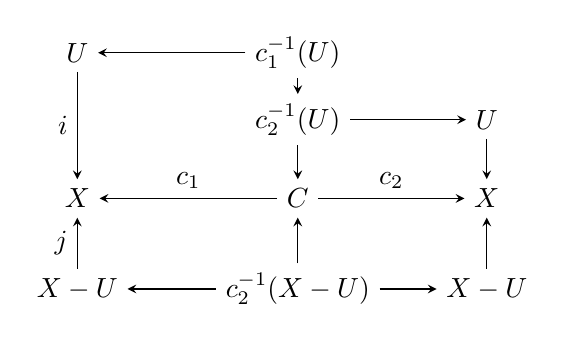
\begin{tikzpicture}[baseline=(current bounding box.center),>=stealth]
\node (U1) at (0,3.0) {$U$};
\node (C1U) at (2.8,3.0) {$c_1^{-1}(U)$};
\node (C2U) at (2.8,2.15) {$c_2^{-1}(U)$};
\node (U2) at (5.2,2.15) {$U$};
\node (X1) at (0,1.15) {$X$};
\node (C) at (2.8,1.15) {$C$};
\node (X2) at (5.2,1.15) {$X$};
\node (XU1) at (0,0) {$X-U$};
\node (C2XU) at (2.8,0) {$c_2^{-1}(X-U)$};
\node (XU2) at (5.2,0) {$X-U$};
\draw[->] (C1U) -- (U1);
\draw[->] (C1U) -- (C2U);
\draw[->] (C2U) -- (U2);
\draw[->] (U1) -- node[left] {$i$} (X1);
\draw[->] (U2) -- (X2);
\draw[->] (C2U) -- (C);
\draw[->] (C2XU) -- (C);
\draw[->] (C) -- node[above] {$c_1$} (X1);
\draw[->] (C) -- node[above] {$c_2$} (X2);
\draw[->] (XU1) -- node[left] {$j$} (X1);
\draw[->] (XU2) -- (X2);
\draw[->] (C2XU) -- (XU1);
\draw[->] (C2XU) -- (XU2);
\end{tikzpicture}
\tag{6.14.1}
\end{equation}
迹态射
\[
\Tr_{c_2}:c_{2!}\Lambda_C\longrightarrow \Lambda_X
\]
于是定义滤过 $G$-等变对应
\begin{equation}
\underline c\in\Hom(c_1^*\Lambda_X,c_2^!\Lambda_X),
\tag{6.14.2}
\end{equation}
其中 $\Lambda_X$ 带有由子模 $i_!\Lambda_U$ 定义的滤过, 即
\[
F^n\Lambda_X=\Lambda_X\quad(n\le0),\qquad
F^1\Lambda_X=i_!\Lambda_U,\qquad
F^n\Lambda_X=0\quad(n\ge1).
\]
相伴分次对象由两个 $G$-等变对应组成
\[
\operatorname{gr}^0\underline c=\underline c_{X-U,X}
\in\Hom(c_1^*\Lambda_{X-U,X},c_2^!\Lambda_{X-U,X}),
\]
\begin{equation}
\operatorname{gr}^1\underline c=\underline c_{U,X}
\in\Hom(c_1^*\Lambda_{U,X},c_2^!\Lambda_{X-U,X}),
\tag{6.14.3}
\end{equation}
这里置
\[
\Lambda_{X-U,X}=j_*\Lambda_{X-U},\qquad
\Lambda_{U,X}=i_!\Lambda_U.
\]
有
\begin{equation}
\underline c_{X-U,U}=j_*\underline c_{X-U},
\tag{6.14.4}
\end{equation}
其中
\[
\underline c_{X-U}\in\Hom(c_1^*\Lambda_{X-U},c_2^!\Lambda_{X-U})
\]
为 $\Tr_{c_2,X-U}$ 定义的对应. 需要指明基环时, 使用记号 $\underline c$, $\underline c_{U,X}$ 等.

遗忘 $G$ 的作用, 有局部项
\begin{equation}
\Tr_{\Lambda}(\underline c),\quad
\Tr_{\Lambda}(\underline c_{U,X}),\quad
\Tr_{\Lambda}(\underline c_{X-U,X})
\in H^0(X^c,K_{X^c}),
\tag{6.14.5}
\end{equation}
由迹的可加性 (III 4.13.1), 它们满足关系
\begin{equation}
\Tr_{\Lambda}(\underline c)
=
\Tr_{\Lambda}(\underline c_{U,X})
+
\Tr_{\Lambda}(\underline c_{X-U,X}).
\tag{6.14.6}
\end{equation}
而且, 由 6.14.4,
\begin{equation}
\Tr_{\Lambda}(\underline c_{X-U,X})
=
j_*^c\Tr_{\Lambda}(\underline c_{X-U}),
\tag{6.14.7}
\end{equation}
其中
\[
j_*^c:H^0((X-U)^c,K_{(X-U)^c})\longrightarrow H^0(X^c,K_{X^c})
\]
为 $j^c:(X-U)^c\to X^c$ 定义的正像态射. 回顾 (III 4.3), 若 $X$ 光滑, $c$ 为闭浸入, $X^c$ 有限, 则 $\Tr_{\Lambda}(\underline c)$ 是 $C$ 与对角线的相交重数 $(C\cdot X)$ 在 $\Lambda$ 中的像. 若再有 $X-U$ 光滑, 则 $\Tr_{\Lambda}(\underline c_{X-U})$ 为 $(c_2^{-1}(X-U)\cdot(X-U))$ 在 $\Lambda$ 中的像. 还注意到, 若 $X-U$ 在 $S$ 上固有, 且 $c|X-U$ 为对角线, 则 Lefschetz 公式 (III 4.7) 蕴含
\[
\int_{X-U}\Tr(\underline c_{X-U})\in\Lambda
\]
是 $X-U$ 的取值于 $\Lambda$ 的 Euler--Poincaré 示性数.

\subsection*{6.15}
设有 $G$-等变图 6.11.1, 其中 $f$, $c$, $d$ 固有, 并有等变开浸入 $U\to X$. 假定 $c_2$ 拟有限且具有有限 Tor 维数,
\[
c_1^{-1}(U)\subset c_2^{-1}(U),
\]
$G$ 在 $C$ 和 $D$ 上平凡作用, 且
\[
f|U:U\longrightarrow f(U)=V
\]
为群为 $G$ 的平展 Galois 覆盖. 最后一条假设蕴含
\[
Rf_*(\Lambda_{U,X})\in\Ob D_{\mathrm{ctf}}({}_{\Lambda[G]}Y):
\]
事实上, $Rf_*(\Lambda_{U,X})$ 集中于 $0$ 次, 并且是 $V$ 上一个局部同构于 $\Lambda[G]$ 的层的零延拓. 因此可对 $L=\Lambda_{U,X}$, $u=\underline c_{U,X}$ 应用 6.12, 结合 6.14.6 和 6.14.7, 得到:

\begin{statement}{命题 6.16}
在 6.15 的假设下, 对每个 $g\in G$ 有
\begin{equation}
f_*^{gc}\Tr_{\Lambda}(g\underline c)
-(fj)_*^{gc}\Tr_{\Lambda}(g\underline c_{X-U})
=
|Z_g|\,\Tr_{\Lambda[G]}(f_*\underline c_{U,X})(g^{-1}),
\tag{6.16.1}
\end{equation}
其中 $j:X-U\to X$ 为包含, $Z_g$ 表示 $g$ 的中心化子.
\end{statement}

对对应的射影系 $\underline c_{\ell}=(\underline c_{\Lambda_n})$ 应用 6.16, 这里 $\Lambda_n=\mathbb Z/\ell^n$, $\ell$ 为不同于 $p$ 的素数; 考虑到 6.14.6 和 6.14.7 取极限并施行 $f_*^{gc}$ 后给出
\[
f_*^{gc}\Tr_{\mathbb Z_{\ell}}(g\underline c_{\ell})
=
f_*^{gc}\Tr_{\mathbb Z_{\ell}}(g\underline c_{\ell,U,X})
+(fj)_*^{gc}\Tr_{\mathbb Z_{\ell}}(g\underline c_{\ell,X-U}),
\]
由 6.13 推出:

\begin{statement}{推论 6.17}
在 6.15 的假设下, 对每个 $g\in G$ 有
\begin{equation}
f_*^{gc}\Tr_{\mathbb Z_{\ell}}(g\underline c_{\ell})
-(fj)_*^{gc}\Tr_{\mathbb Z_{\ell}}(g\underline c_{\ell,X-U})
=
|Z_g|\,\Tr_{\mathbb Z_{\ell}[G]}(f_*\underline c_{\ell,U,X})(g^{-1}),
\tag{6.17.1}
\end{equation}
这里采用 6.16 的记号.
\end{statement}

根据局部迹与局部化的相容性及 6.14 的说明, 可见当 (XII 4.5) 中考虑的 $G$ 的自同态 $\varphi$ 为恒等映射时, 6.17 以更一般的表述肯定地解决了 Grothendieck 的整除性猜想.

事实上, 沿用 5.13 的方法, 不难在以下情形给出类似于 6.12、6.13、6.16、6.17 的整除性陈述: $c$ 不一定 $G$-等变, 但 $c_2$ 等变, 而 $c_1$ 对 $G$ 的每个点 $x$ 满足
\[
c_1(xg)=c_1(x)\varphi(g)
\]
其中 $\varphi$ 为给定的 $G$ 的自同态. 此时整除公式仍按上述方式书写, 只需用 $g^{-1}$ 的 $\varphi$-中心化子替换 $Z_g$ (5.13.5).

\subsection*{6.18}
置
\begin{equation}
N_G=\sum_{g\in G} g\in\Lambda[G].
\tag{6.18.1}
\end{equation}
设 $X$ 为 $S$-概形. 对 $L\in\Ob D({}_{\Lambda[G]}X)$, 左乘 $N_G$ 诱导 $D(X)$ 中的箭头
\begin{equation}
N_G:\Lambda\lten_{\Lambda[G]}L
\longrightarrow
\RHom_{\Lambda[G]}(\Lambda,L),
\tag{6.18.2}
\end{equation}
其中 $\Lambda$ 经由将每个 $g\in G$ 映到 $1$ 的自然增广视为 $\Lambda[G]$-代数.

\begin{statement}{引理 6.18.3}
若 $L\in\Ob D_{\mathrm{ctf}}({}_{\Lambda[G]}X)$, 则箭头 6.18.2 为同构.
\end{statement}

经分步归约, 先归结为 $L$ 完美, 再归结为 $L=\Lambda[G]$; 此时断言由 $N_G$ (6.18.1) 是左 $\Lambda[G]$-模 $\Lambda[G]$ 的 $G$-不变元模的一组基这一事实推出.

\begin{statement}{命题 6.19}
在 6.11 的情形下, 设 $M\in\Ob D_{\mathrm{ctf}}(Y)$,
\[
v\in\Hom(d_1^*M,d_2^!M),
\]
设 $a:M\to f_*L$ 为 $D({}_{\Lambda[G]}Y)$ 中的箭头, 其中 $M$ 经增广 $\Lambda[G]\to\Lambda$ 视为 $D({}_{\Lambda[G]}Y)$ 的对象, 使方块
\[
\begin{tikzcd}[column sep=large,row sep=large]
d_1^*M \arrow[r,"v"] \arrow[d] & d_2^!M \arrow[d] & {}\\
d_1^*f_*L \arrow[r,"f_*u"'] & d_2^!f_*L
\end{tikzcd}
\]
交换. 假定 $f_*M\in\Ob D_{\mathrm{ctf}}({}_{\Lambda[G]}Y)$, 且 $a$ 诱导同构
\[
M\xrightarrow{\sim}\RHom_{\Lambda[G]}(\Lambda,f_*L).
\]
则
\begin{equation}
\Tr_{\Lambda}(v)=
\sum_{g\in G_{\natural}}\Tr_{\Lambda[G]}(f_*u)(g^{-1}).
\tag{6.19.1}
\end{equation}
\end{statement}

由 6.18.3, $a$ 与 $N_G^{-1}$ 复合给出同构
\[
M\xrightarrow{\sim}\Lambda\lten_{\Lambda[G]}f_*L,
\]
在此同构下, $v$ 等同于
\[
\Lambda\lten_{\Lambda[G]}f_*u.
\]
由 6.7.2, $\Tr_{\Lambda}(v)$ 因而为 $\Tr_{\Lambda[G]}(f_*u)$ 在增广
\[
\Lambda[G]\longrightarrow \Lambda.
\]
所诱导的箭头下的像. 此增广按定义将每个共轭类映到 $1$, 故得结论.

\subsection*{6.20}
对 $i=1,2$, 设 $X_i$ 为 $G$-$S$-概形, 且
\[
X=X_1\times_SX_2,\qquad c:C\to X
\]
为 $G$-$S$-态射, 使 $c_2$ 拟有限且具有有限 Tor 维数. 设 $L_i\in\Ob D^+(G,{}_AX_i)$. 迹态射
\[
\Tr_{c_2}:c_{2!}c_2^*L_2\longrightarrow L_2
\]
由伴随性定义 $D(G,X)$ 中的箭头, 仍记作
\begin{equation}
\Tr_{c_2}:c_2^*L_2\longrightarrow c_2^!L_2,
\tag{6.20.1}
\end{equation}
它给每个 $G$-等变态射
\[
u\in\Hom(c_1^*L_1,c_2^*L_2)
\]
赋予 $G$-等变对应
\begin{equation}
u^! = \Tr_{c_2}\circ u\in\Hom(c_1^*L_1,c_2^!L_2).
\tag{6.20.2}
\end{equation}

\begin{statement}{命题 6.21}
设 $f:X\to Y$ 为固有 $G$-态射, 6.11.1 为等变交换方块, $G$ 在 $Y$ 和 $D$ 上平凡作用. 假定 $c$, $d$ 固有, $c_2$, $d_2$ 拟有限且具有有限 Tor 维数, 并且方块
\[
\begin{tikzcd}[column sep=large,row sep=large]
C \arrow[r,"c_2"] \arrow[d,"h"'] & X \arrow[d,"f"]\\
D \arrow[r,"d_2"'] & Y
\end{tikzcd}
\]
为笛卡尔且 Tor 无关 (SGA 6 III 1.5). 设 $M\in\Ob D_{\mathrm{ctf}}(Y)$,
\[
v\in\Hom(d_1^*M,d_2^*M),
\]
从而有 $G$-等变同态
\[
h^*v\in\Hom(c_1^*f^*M,c_2^*f^*M),
\]
及 $G$-等变对应
\[
(h^*v)^!\in\Hom(c_1^*f^*M,c_2^!f^*M),
\qquad
f_*((h^*v)^!)\in\Hom(d_1^*(f_*f^*M),d_2^!(f_*f^*M)).
\]
则有 $D({}_{\Lambda[G]}Y)$ 中箭头的交换方块, 其中以平凡作用将 $M$ 视为 $D({}_{\Lambda[G]}Y)$ 的对象,
\[
\begin{tikzcd}[column sep=huge,row sep=large]
d_1^*M \arrow[r,"v^!"] \arrow[d] & d_2^!M \arrow[d] & {}\\
d_1^*f_*f^*M \arrow[r,"f_*((h^*v)^!)"'] & d_2^!f_*f^*M,
\end{tikzcd}
\]
其中竖直箭头由伴随箭头 $M\to f_*f^*M$ 给出.
\end{statement}

置 $h^*v=u$, $f^*M=L$, 考虑图
\[
\begin{tikzcd}[column sep=large,row sep=large]
d_1^*M \arrow[r,"v"] \arrow[d] &
d_2^*M \arrow[r,"\Tr_{d_2}"] \arrow[d] &
d_2^!M \arrow[d] & {}\\
d_1^*f_*L \arrow[r] &
h_*c_1^*L \arrow[r,"h_*\Tr_{c_2}"] &
h_*c_2^!L \arrow[r] &
d_2^!f_*L .
\end{tikzcd}
\]
箭头 (1)、(3) 由伴随箭头 $M\to f_*L$ 给出, (2) 由伴随箭头 $d_2^*M\to h_*h^*(d_2^*M)=h_*c_2^*L$ 给出, (4) 由换基箭头给出, (5) 为典范同构 (SGA 4 XVIII 3.1.12.3). 按定义, $v^!$ 是上行的复合. 另一方面, 由对应的正像的解释 (III 3.5 b), 3.7), $f_*u^!$ 是下行的复合. 因此只须证明方块 (A) 和 (B) 交换. (A) 的交换性由换基箭头的定义立即得出. 至于 (B), 由于 Tor 无关假设, $\Tr_{d_2}$ 与沿 $f$ 的换基相容 (SGA $4^{1/2}$ Cycle 2.3.3), 故交换.

应用 6.19, 得到:

\begin{statement}{推论 6.22}
在 6.21 的假设下, 假定
\[
f_*f^*M\in\Ob D_{\mathrm{ctf}}({}_{\Lambda[G]}Y),
\]
且伴随箭头
\[
M\to f_*f^*M
\]
诱导同构
\[
M\xrightarrow{\sim}\RHom_{\Lambda[G]}(\Lambda,f_*f^*M).
\]
则
\begin{equation}
\Tr_{\Lambda}(v^!)=
\sum_{g\in G_{\natural}}\Tr_{\Lambda[G]}(f_*((f^*v)^!))(g^{-1}).
\tag{6.22.1}
\end{equation}
\end{statement}

\begin{statement}{命题 6.23}
在 6.21 的假设下, 再假定存在开浸入
\[
i:V\hookrightarrow Y
\]
使 $(fc_1)^{-1}(V)$ 连通, $d_1^{-1}(V)\subset d_2^{-1}(V)$, 且 $f$ 诱导群为 $G$ 的主 Galois 覆盖,
\[
f_V:U=f^{-1}(V)\to V.
\]
还假定 $M$ 形如 $M=i_!E$, $E\in\Ob D(V)$, 并有 $D(G,X)$ 中的同构
\[
\alpha:f_V^*E\xrightarrow{\sim}\Lambda_X\lten_{\Lambda}E_0
\]
其中 $E_0\in\Ob D(\Lambda[G])$, 在 $\Lambda$ 上完美. 设
\[
v\in\Hom(d_1^*M,d_2^*M)
\]
如 6.21, 并设
\[
v_0\in\Hom_{\Lambda[G]}(E_0,E_0)
\]
为借助 $\alpha$ 由 $f^*v|c_1^{-1}(U)$ 定义的同态. 若 $\underline c_{U,X}$ 表示 6.14.3 定义的对应, 采用记号 6.20.2, 则有
\begin{equation}
\Tr_{\Lambda}(v^!)
=
\sum_{g\in G_{\natural}}
\Tr_{\Lambda[G]}(f_*\underline c_{U,X})(g^{-1})\Tr_{\Lambda}(gv_0).
\tag{6.23.1}
\end{equation}
\end{statement}

注意, 由 $\Tr_{\Lambda}$ 的中心性, 右端与 $\alpha$ 的选择无关.

由投影公式
\[
f_*f^*\Lambda_Y\lten M\xrightarrow{\sim}f_*f^*M
\]
及 6.15, $M$ 满足 6.22 的假设. 另一方面, $\alpha$ 定义同构
\[
f^*M\xrightarrow{\sim}\Lambda_{U,X}\otimes E_0
\]
在此同构下, $(f^*v)^!$ 等同于外张量积 $\underline c_{U,X}\otimes v_0$. 由投影公式, $f_*f^*M$ 因而等同于 $f_*(\Lambda_{U,X})\otimes E_0$, 而 $f_*((f^*v)^!)$ 等同于外张量积 $f_*\underline c_{U,X}\otimes v_0$. 对 $g\in G$, $Z_g$-等变对应 $gf_*((f^*v)^!)$ 因而等同于
\[
gf_*\underline c_{U,X}\otimes gv_0.
\]
由于 6.10.4 给出
\[
\Tr_{\Lambda[G]}(f_*((f^*v)^!))(g^{-1})
=
\Tr_{\Lambda[Z_g]}(gf_*((f^*v)^!))(e),
\]
结合 6.22.1, 只需证明公式
\[
\Tr_{\Lambda[Z_g]}(gf_*\underline c_{U,X}\otimes gv_0)(e)
=
\Tr_{\Lambda[G]}(f_*\underline c_{U,X})(g^{-1})\Tr_{\Lambda}(gv_0),
\]
或者由 6.10.4 等价地证明
\begin{equation}
\Tr_{\Lambda[Z_g]}(gf_*\underline c_{U,X}\otimes gv_0)(e)
=
\Tr_{\Lambda[Z_g]}(gf_*\underline c_{U,X})(e)\Tr_{\Lambda}(gv_0).
\tag{6.23.2}
\end{equation}
必要时以 $Z_g$ 替换 $G$, 可假定 $g=e$. 回到迹的定义, 可见只需建立以下引理.

\begin{statement}{引理 6.23.3}
(参见 SGA $4^{1/2}$ Report 4.7). 设 $P$ 为局部是有限型自由模的直和因子的 $G_V$-模, $P'=i_!P$, $Q$ 为在 $\Lambda$ 上完美的 $\Lambda[G]$-模复形. 则以 $G$ 的对角作用将 $P\lten_{\Lambda}Q$ 视为 $D({}_{\Lambda[G]}V)$ 的对象时, 它在 $\Lambda[G]$ 上完美, 并有交换方块
\begin{equation}\tag{*}
\begin{tikzcd}[column sep=huge,row sep=large]
\delta^*\RHom_{\Lambda[G]}(p_1^*P',p_2^!P')\lten_{\Lambda}
\RHom_{\Lambda[G]}(Q,Q) \arrow[r,"(1)"] \arrow[d,"(2)"']
& K_Y \arrow[d,equal]\\
\delta^*\RHom_{\Lambda[G]}(p_1^*P'\lten_{\Lambda}Q,p_2^!P'\lten_{\Lambda}Q) \arrow[r,"(3)"']
& K_Y ,
\end{tikzcd}
\end{equation}
其中 $\delta:Y\to Y\times_SY$ 为对角线, 上水平箭头为以下箭头的张量积
\[
\delta^*\RHom_{\Lambda[G]}(p_1^*P',p_2^!P')\xrightarrow{6.5.3}
K\Lambda[G]_{Y,\natural}\xrightarrow{x\mapsto x(e)}K_Y
\]
以及
\[
\RHom_{\Lambda[G]}(Q,Q)\xrightarrow{\Tr_{\Lambda}}\Lambda,
\]
竖直箭头由外张量积沿对角线
\[
\Lambda[G]\to\Lambda[G]\otimes\Lambda[G],
\]
作限制得到, 下水平箭头为 6.5.3 (因 $P'\lten_{\Lambda}Q\in\ob D_{\mathrm{ctf}}({}_{\Lambda[G]}Y)$ 而有定义) 与 $x\mapsto x(e)$ 的复合.\footnote{应当可以用 ($\Lambda[G]$ 上的) 完美复形替换 $P$ (甚至用 $D_{\mathrm{ctf}}({}_{\Lambda[G]}Y)$ 的对象替换 $P'$).}
\end{statement}

第一条断言显然, 因为可归结为 $P=\Lambda[G]_V$, 此时 $P\lten_{\Lambda}Q$ 同构于 $P$ 与赋予 $G$ 平凡作用的 $Q$ 的张量积. 对第二条断言, 先注意由 6.5.4 和 6.5.5 有
\[
\delta^*\RHom_{\Lambda[G]}(p_1^*P',p_2^!P')
\xrightarrow{\sim}
D_{\Lambda[G]}(i_!P)\lten_{\Lambda[G]} i_!P
\xrightarrow{\sim}
i_!(D_{\Lambda[G]}P\lten_{\Lambda[G]}P),
\]
故只须验证 (*) 在 $V$ 上诱导的方块交换. 因此可假定 $V=Y$. 此时方块 (*) 写为
\begin{equation}\tag{**}
\begin{tikzcd}[column sep=huge,row sep=large]
\RHom_{\Lambda[G]}(P,K_Y\lten P)\lten\RHom_{\Lambda[G]}(Q,Q) \arrow[r,"(1)"] \arrow[d,"(2)"']
& K_Y \arrow[d,equal]\\
\RHom_{\Lambda[G]}(P\lten Q,K_Y\lten P\lten Q) \arrow[r,"(3)"']
& K_Y ,
\end{tikzcd}
\end{equation}
其中 (2) 为外张量积, (1) 由
\[
\Tr_{\Lambda[G]}(-)(e)\otimes\Tr_{\Lambda},
\]
给出 (迹按第~5 节的意义理解), (3) 由 $\Tr_{\Lambda[G]}(-)(e)$ 给出. 经下降归结为 $P=\Lambda[G]_Y$; 根据开头的说明, 此时可假定 $G$ 在 $Q$ 上平凡作用. 断言于是由 5.12.5 立即推出.

\subsection*{6.24}
若 $\Lambda$ 被某个素数 $\ell\ne p$ 的幂零化, 则 6.23.1 的右端可改写为
\[
\sum_{g\in G_{\natural}}
\Tr_{\mathbb Z_{\ell}[G]}(f_*\underline c_{\ell,U,X})(g^{-1})
\Tr_{\Lambda}(gv_0),
\]
这里采用 6.17 的记号. 公式 6.17.1 表明, Grothendieck 在 (XII 6.2) 定义的局部项与 Verdier 的局部项一致, 至少当该处所考虑的 $G$ 的自同态 $\varphi$ 为恒等映射时如此; 但如前所述, 这个限制并不严重. 若 $Y$ 在 $S$ 上固有, 则将 6.23.1 与 $Y\to S$ 的 Lefschetz 公式 (III 4.7) 结合, 得到推广 (XII 6.3) 的公式, 因而也推广 (SGA $4^{1/2}$ Report) 及本报告第一部分所证明的 Frobenius 的 Lefschetz 公式.

\section*{参考文献}

\begin{enumerate}[label={[\arabic*]}]
\item Cartan, H. and Eilenberg, S. -- \textit{Homological Algebra}, Princeton University Press, 1956.
\item Grothendieck, A. -- Formule de Lefschetz et rationalité des fonctions $L$, Séminaire Bourbaki 64/65, no. 279, in \textit{Dix exposés sur la cohomologie des schémas}, North Holland, Pub. Co., 1968.
\item Illusie, L. -- Complexe cotangent et déformations I, II, Lecture Notes in Mathematics 239, 283, Springer-Verlag, 1971, 1972.
\item Langlands, R. P. -- Modular forms and $\ell$-adic representations, in \textit{Modular Functions of One Variable II}, Lecture Notes in Mathematics 349, Springer-Verlag, 1973.
\item Stallings, J. -- Centerless groups -- an algebraic formulation of Gottlieb's theorem, \textit{Topology} 4, p. 129--134, 1965.
\item Verdier, J.-L. -- The Lefschetz fixed point formula in étale cohomology, in \textit{Proceedings of a conference on local fields}, Springer-Verlag, 1967.
\end{enumerate}

SGA $4^{1/2}$: \textit{Cohomologie étale}, P. Deligne 著, Lecture Notes in Mathematics 569, Springer-Verlag, 1977.

在 SGA $4^{1/2}$ 中:
\[
\text{Finiteness Theorem: }\ell\text{ 进上同调中的有限性定理;}
\]
\[
\text{Cycle: 与闭链相伴的上同调类;}
\]
\[
\text{Report: 关于迹公式的报告.}
\]

